% Options for packages loaded elsewhere

\PassOptionsToPackage{unicode}{hyperref}
\PassOptionsToPackage{hyphens}{url}
%
\documentclass{rgclass}

\usepackage{lmodern}
\usepackage{longtable}
\usepackage{float}
\usepackage{arydshln}
\usepackage{placeins}

% Use upquote if available, for straight quotes in verbatim environments
\IfFileExists{upquote.sty}{\usepackage{upquote}}{}
\IfFileExists{microtype.sty}{% use microtype if available
  \usepackage[]{microtype}
  \UseMicrotypeSet[protrusion]{basicmath} % disable protrusion for tt fonts
}{}
\makeatletter
\@ifundefined{KOMAClassName}{% if non-KOMA class
  \IfFileExists{parskip.sty}{%
    \usepackage{parskip}
  }{% else
    \setlength{\parindent}{0pt}
    \setlength{\parskip}{6pt plus 2pt minus 1pt}}
}{% if KOMA class
  \KOMAoptions{parskip=half}}
\makeatother
\usepackage{xcolor}
\IfFileExists{xurl.sty}{\usepackage{xurl}}{} % add URL line breaks if available
\IfFileExists{bookmark.sty}{\usepackage{bookmark}}{\usepackage{hyperref}}
\urlstyle{same} % disable monospaced font for URLs
\usepackage{color}
\usepackage{fancyvrb}
\newcommand{\VerbBar}{|}
\newcommand{\VERB}{\Verb[commandchars=\\\{\}]}
\DefineVerbatimEnvironment{Highlighting}{Verbatim}{commandchars=\\\{\}}
% Add ',fontsize=\small' for more characters per line
\usepackage{framed}
\definecolor{shadecolor}{RGB}{248,248,248}
\newenvironment{Shaded}{\begin{snugshade}}{\end{snugshade}}
\newcommand{\AlertTok}[1]{\textcolor[rgb]{0.94,0.16,0.16}{#1}}
\newcommand{\AnnotationTok}[1]{\textcolor[rgb]{0.56,0.35,0.01}{\textbf{\textit{#1}}}}
\newcommand{\AttributeTok}[1]{\textcolor[rgb]{0.77,0.63,0.00}{#1}}
\newcommand{\BaseNTok}[1]{\textcolor[rgb]{0.00,0.00,0.81}{#1}}
\newcommand{\BuiltInTok}[1]{#1}
\newcommand{\CharTok}[1]{\textcolor[rgb]{0.31,0.60,0.02}{#1}}
\newcommand{\CommentTok}[1]{\textcolor[rgb]{0.56,0.35,0.01}{\textit{#1}}}
\newcommand{\CommentVarTok}[1]{\textcolor[rgb]{0.56,0.35,0.01}{\textbf{\textit{#1}}}}
\newcommand{\ConstantTok}[1]{\textcolor[rgb]{0.00,0.00,0.00}{#1}}
\newcommand{\ControlFlowTok}[1]{\textcolor[rgb]{0.13,0.29,0.53}{\textbf{#1}}}
\newcommand{\DataTypeTok}[1]{\textcolor[rgb]{0.13,0.29,0.53}{#1}}
\newcommand{\DecValTok}[1]{\textcolor[rgb]{0.00,0.00,0.81}{#1}}
\newcommand{\DocumentationTok}[1]{\textcolor[rgb]{0.56,0.35,0.01}{\textbf{\textit{#1}}}}
\newcommand{\ErrorTok}[1]{\textcolor[rgb]{0.64,0.00,0.00}{\textbf{#1}}}
\newcommand{\ExtensionTok}[1]{#1}
\newcommand{\FloatTok}[1]{\textcolor[rgb]{0.00,0.00,0.81}{#1}}
\newcommand{\FunctionTok}[1]{\textcolor[rgb]{0.00,0.00,0.00}{#1}}
\newcommand{\ImportTok}[1]{#1}
\newcommand{\InformationTok}[1]{\textcolor[rgb]{0.56,0.35,0.01}{\textbf{\textit{#1}}}}
\newcommand{\KeywordTok}[1]{\textcolor[rgb]{0.13,0.29,0.53}{\textbf{#1}}}
\newcommand{\NormalTok}[1]{#1}
\newcommand{\OperatorTok}[1]{\textcolor[rgb]{0.81,0.36,0.00}{\textbf{#1}}}
\newcommand{\OtherTok}[1]{\textcolor[rgb]{0.56,0.35,0.01}{#1}}
\newcommand{\PreprocessorTok}[1]{\textcolor[rgb]{0.56,0.35,0.01}{\textit{#1}}}
\newcommand{\RegionMarkerTok}[1]{#1}
\newcommand{\SpecialCharTok}[1]{\textcolor[rgb]{0.00,0.00,0.00}{#1}}
\newcommand{\SpecialStringTok}[1]{\textcolor[rgb]{0.31,0.60,0.02}{#1}}
\newcommand{\StringTok}[1]{\textcolor[rgb]{0.31,0.60,0.02}{#1}}
\newcommand{\VariableTok}[1]{\textcolor[rgb]{0.00,0.00,0.00}{#1}}
\newcommand{\VerbatimStringTok}[1]{\textcolor[rgb]{0.31,0.60,0.02}{#1}}
\newcommand{\WarningTok}[1]{\textcolor[rgb]{0.56,0.35,0.01}{\textbf{\textit{#1}}}}
\usepackage{graphicx}
\makeatletter
\def\maxwidth{\ifdim\Gin@nat@width>\linewidth\linewidth\else\Gin@nat@width\fi}
\def\maxheight{\ifdim\Gin@nat@height>\textheight\textheight\else\Gin@nat@height\fi}
\makeatother

\usepackage{lineno}\linenumbers
\usepackage{xcolor}
\usepackage{bm}
\ifLuaTeX
  \usepackage{selnolig}  % disable illegal ligatures
\fi

\usepackage{hyperref}
\hypersetup{
    colorlinks=true, %set true if you want colored links
    linktoc=all,     %set to all if you want both sections and subsections linked
    linkcolor=blue,  %choose some color if you want links to stand out
    citecolor=blue
}

\gdef\thesection{S\arabic{section}}
\gdef\thefigure{S\arabic{figure}}
\gdef\thetable{S\arabic{table}}
\renewcommand{\theequation}{S\arabic{equation}}

\begin{document}

\noindent \normalsize{{\it Methods in Ecology and Evolution}}\\
%\normalsize{Running head: Multistate Langevin diffusion}\\[0.6cm]
\LARGE On steps and turns: 
  hidden Markov model formulations for inferring animal movement behavior\\
\large{Brett T.\ McClintock}

%\tableofcontents

\newpage

%\section{Realized steps and turns from simulation scenarios}
\begin{figure}
    \centering
    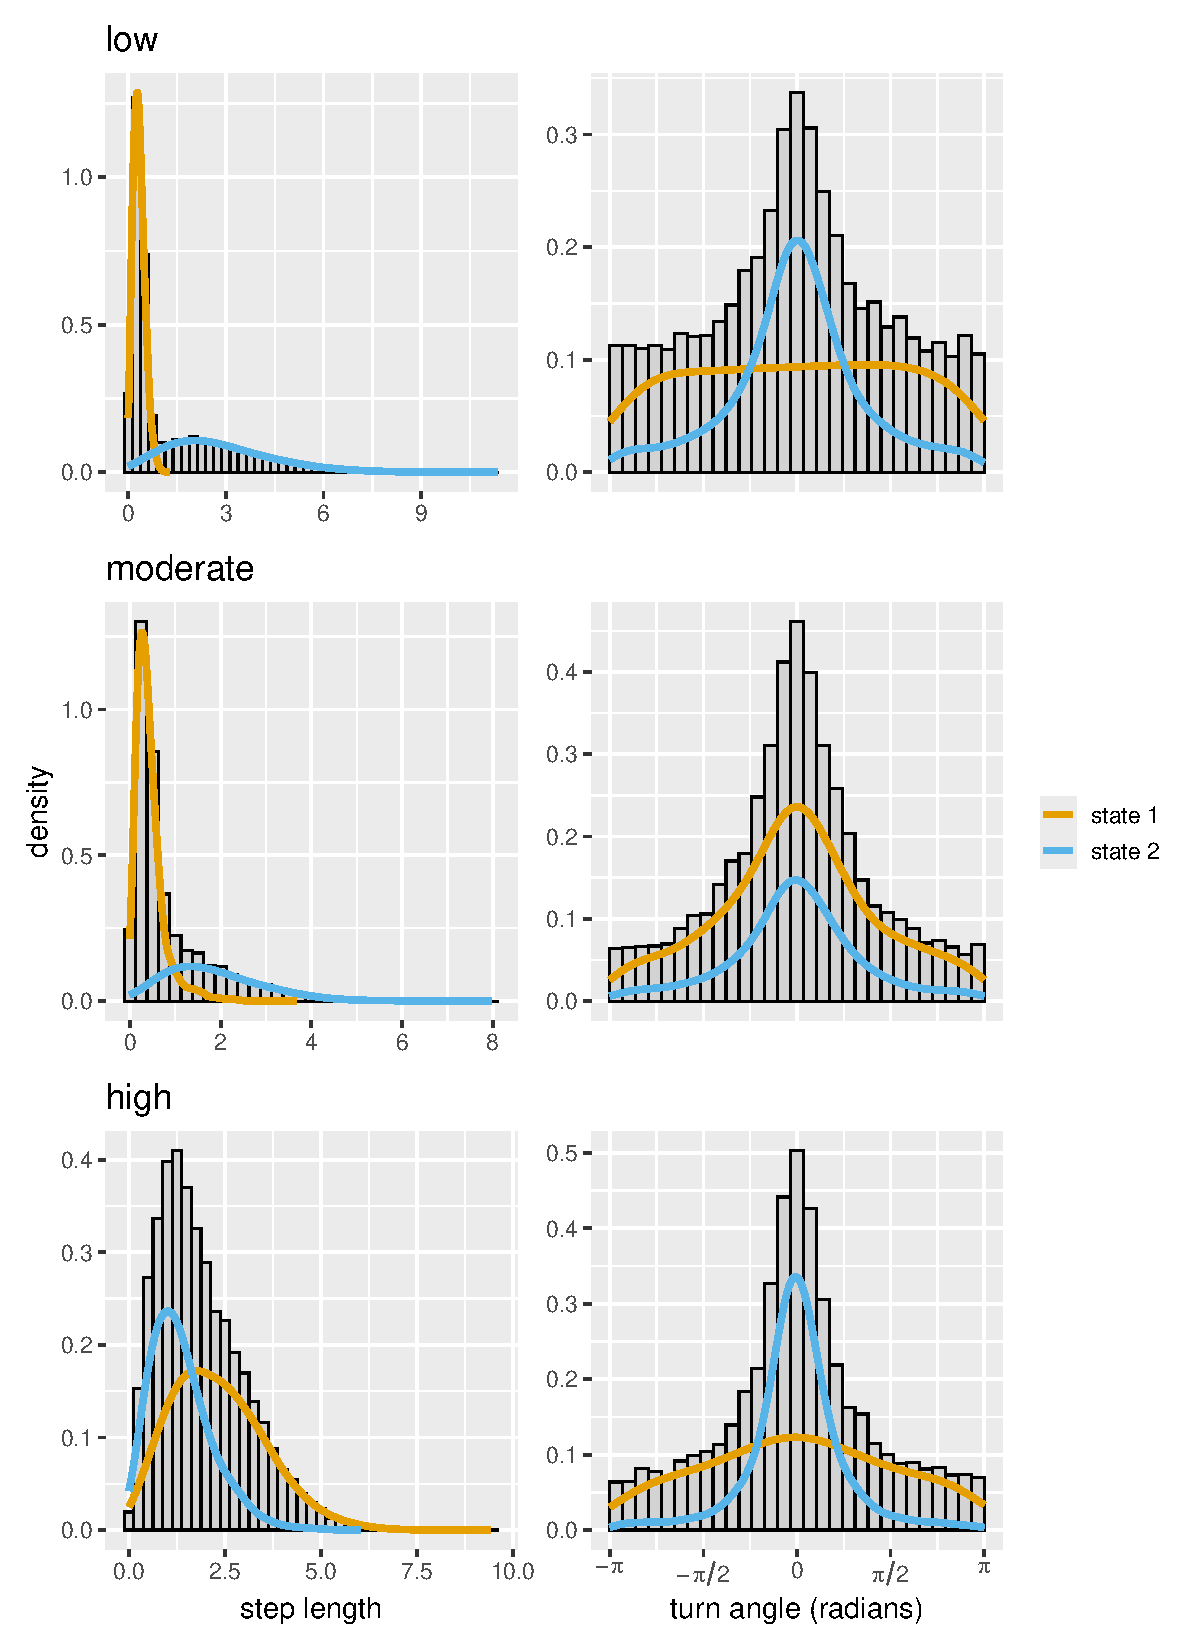
\includegraphics[width=.75\textwidth]{../simulations/crwSTDensPlots.pdf}
    \caption{Realized step lengths and turn angles for a single dataset generated from a 2-state correlated step and turn model with ``low'' (top row), ``moderate'' (middle row), and ``high'' (bottom row) levels of overlap in the state-dependent observation distributions. State-dependent curves were computed using a Gaussian kernel density estimator.}
    \label{fig:crwSTDensPlots}
\end{figure}

\begin{figure}
    \centering
    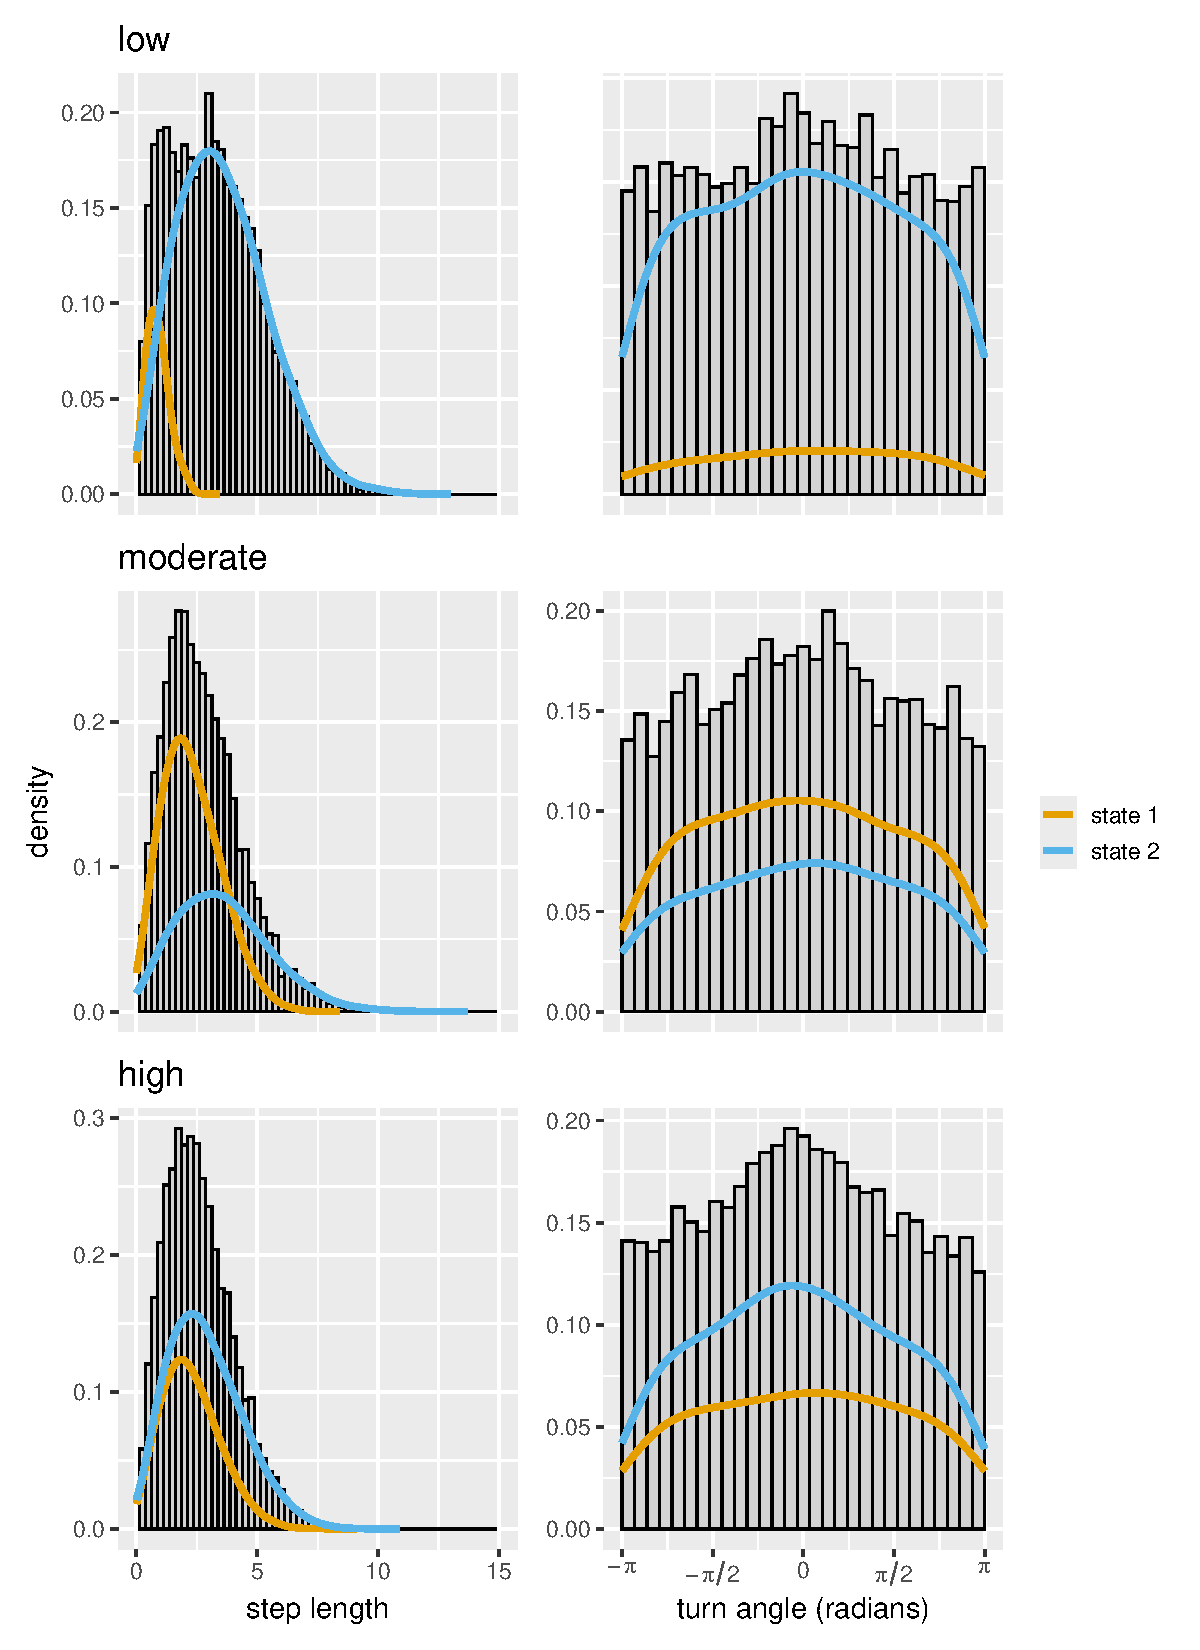
\includegraphics[width=.75\textwidth]{../simulations/spatialStudyplotDens.pdf}
    \caption{Realized step lengths and turn angles for a single dataset generated from a 2-state Langevin-based model with ``low'' (top row), ``moderate'' (middle row), and ``high'' (bottom row) levels of overlap in the state-dependent observation distributions. State-dependent curves were computed using a Gaussian kernel density estimator.}
    \label{fig:spatialStudyplotDens}
\end{figure}


\begin{figure}
    \centering
    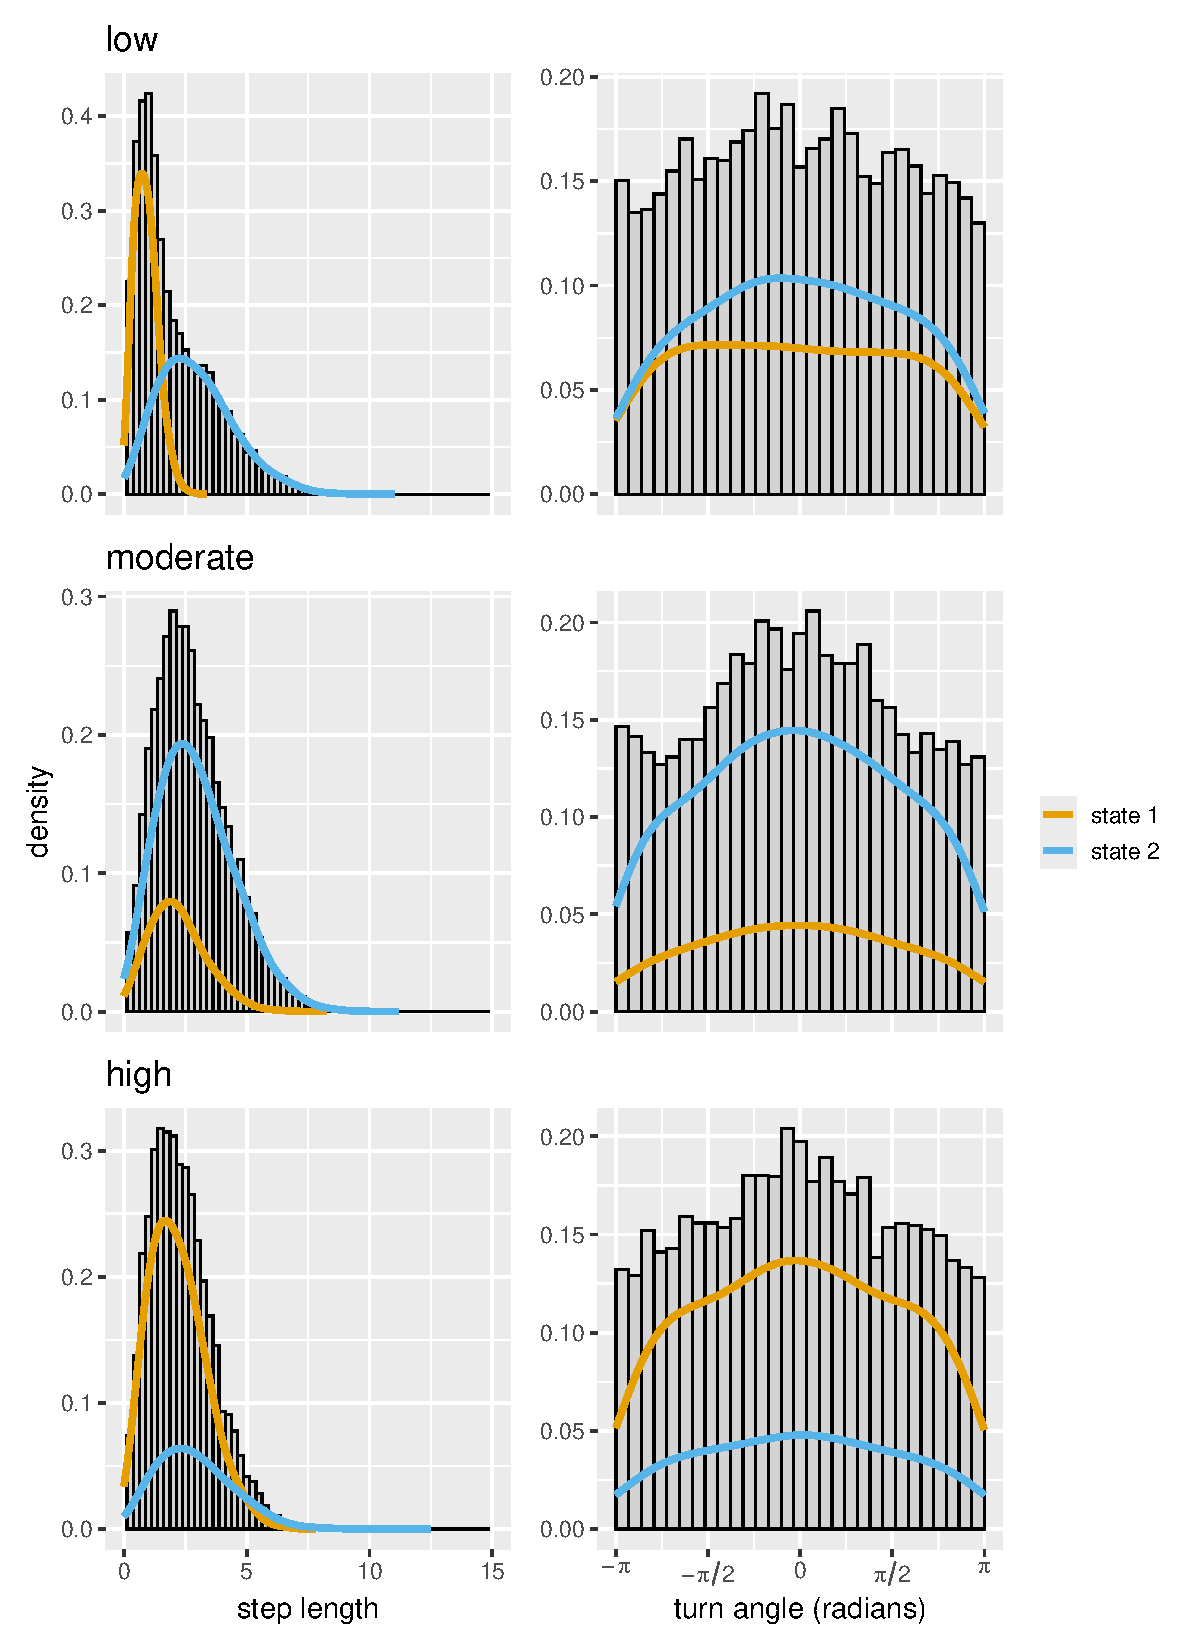
\includegraphics[width=.75\textwidth]{../simulations/spatialStudyplotDens_noLangevin.pdf}
    \caption{Realized step lengths and turn angles for a single dataset generated from a 2-state potential function model with ``low'' (top row), ``moderate'' (middle row), and ``high'' (bottom row) levels of overlap in the state-dependent observation distributions. State-dependent curves were computed using a Gaussian kernel density estimator.}
    \label{fig:spatialStudyplotDens}
\end{figure}

\begin{figure}
    \centering
    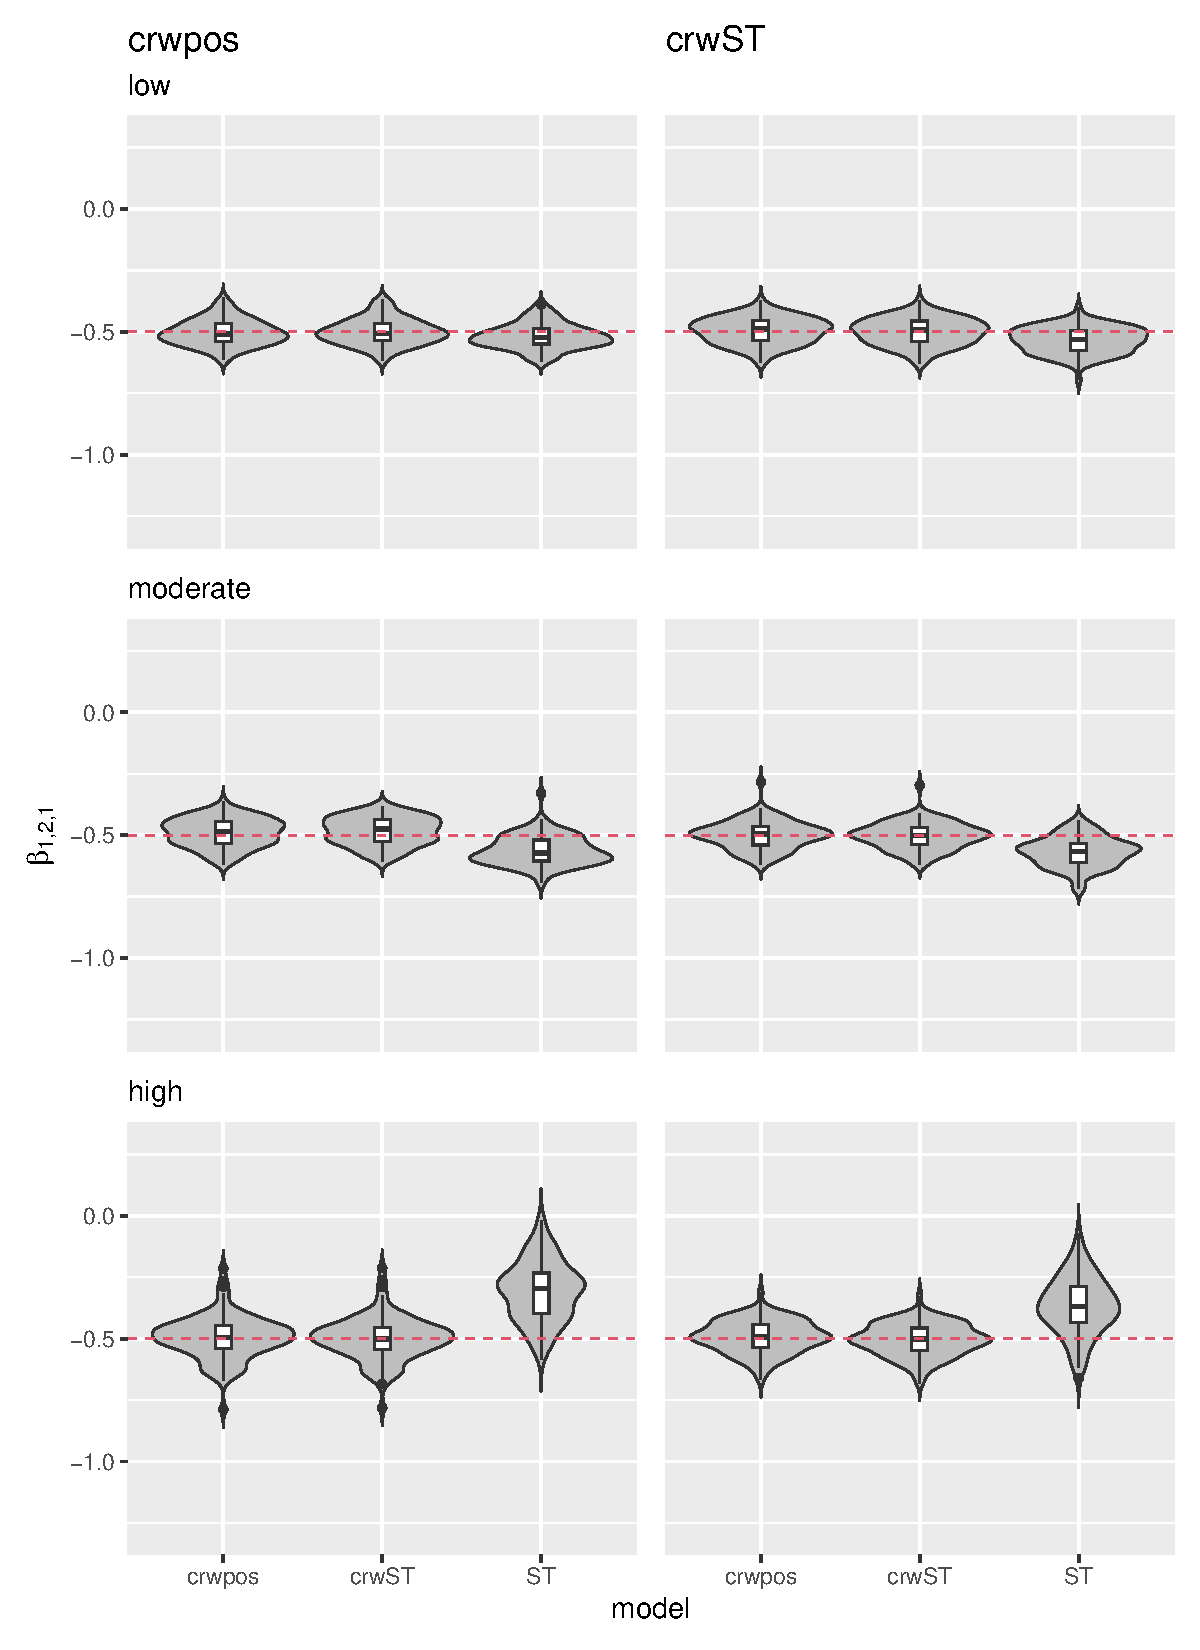
\includegraphics[width=0.9\textwidth]{../simulations/crwBeta12Plots.pdf}
    \caption{Violin plots for the estimated environmental covariate effect on transitions from state 1 to state 2 $(\beta_{12})$ from 100 simulations with data generated from a 2-state correlated random walk HMM in the Cartesian plane (``crwpos''; left column) and a correlated step and turn HMM in the polar plane (``crwST''; right column), with three degrees of overlap in the state-dependent observation distributions: ``low'' (top row), ``moderate'' (middle row), and ``high'' (bottom row). 
    Three models were fitted to each simulated dataset: 1) ``crwpos''; 2) ``crwST''; and 3) the standard 2-state step and turn HMM (``ST'').}
    \label{fig:crwBeta12Plots}
\end{figure}

\begin{figure}
    \centering
    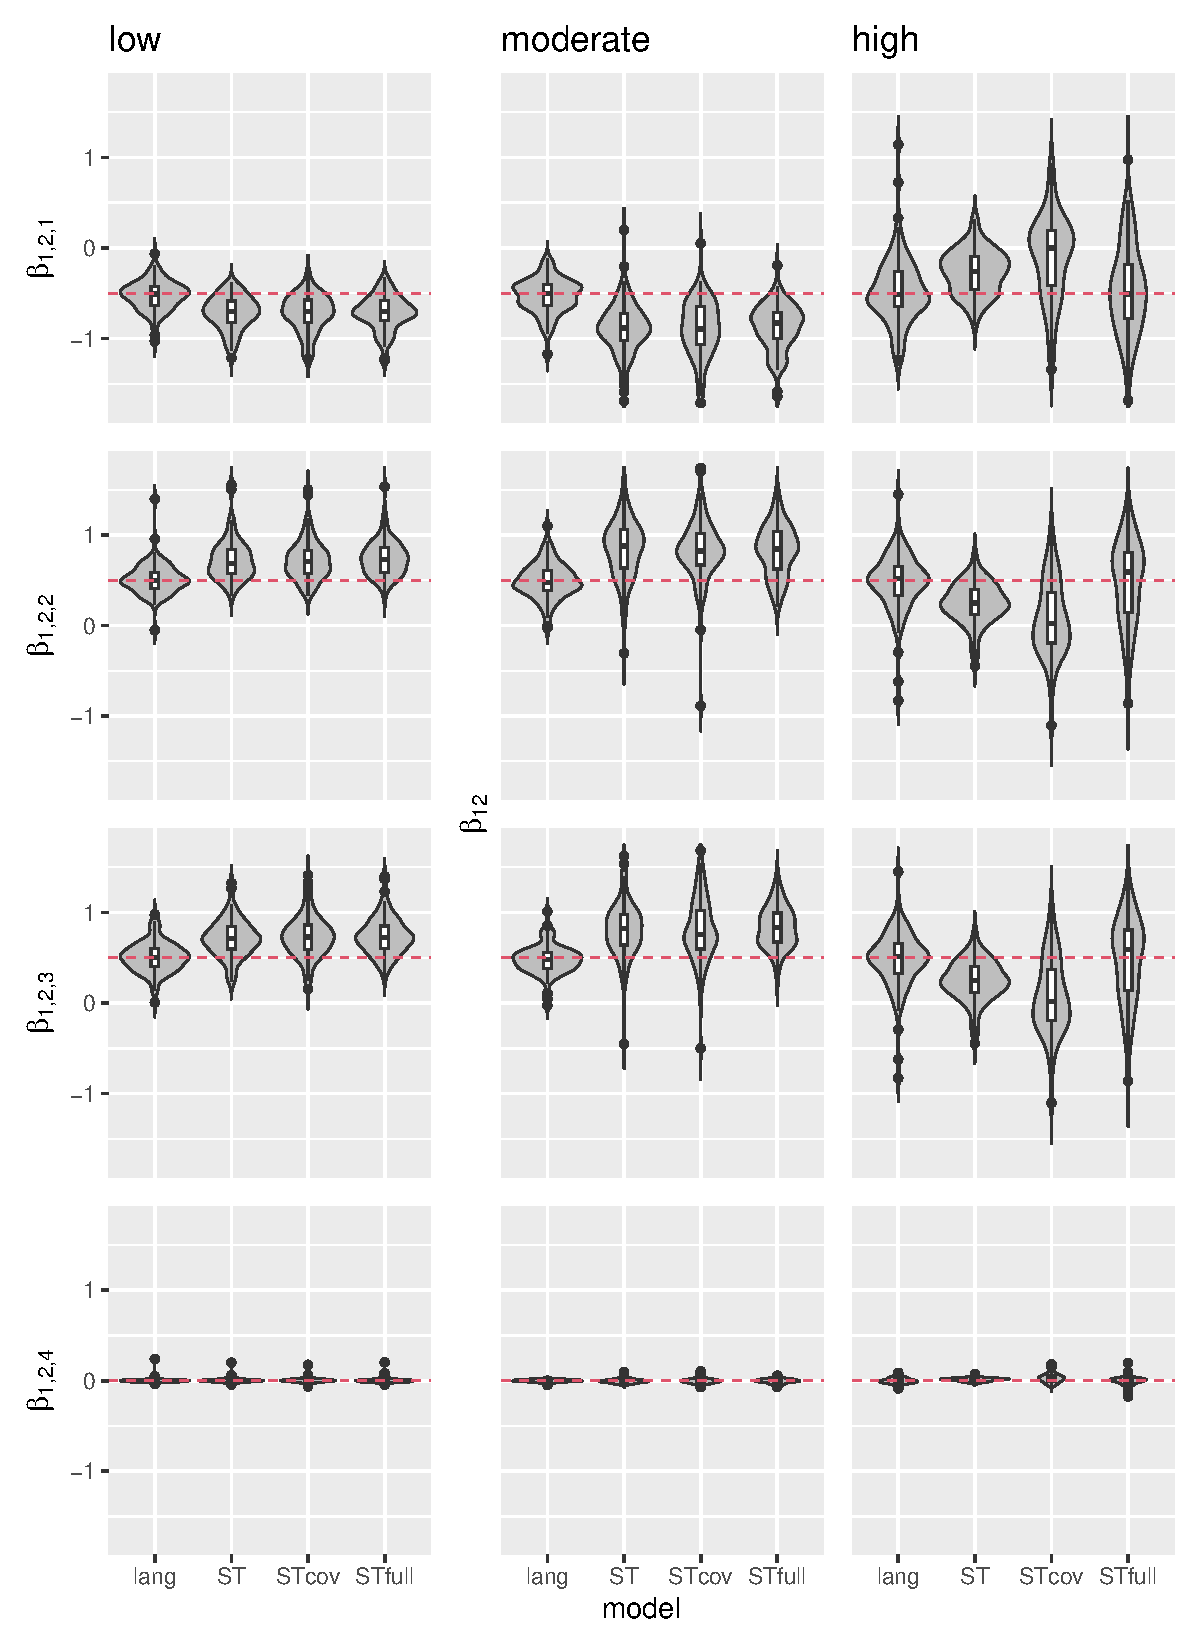
\includegraphics[width=0.8\textwidth]{../simulations/spatBeta12Plots.pdf}
    \caption{Violin plots for the estimated environmental covariate effects on transitions from state 2 to state 1 $\left(\beta_{1,2,k};k=1,\ldots,4\right)$ from 100 simulations with data generated from a 2-state Langevin-based HMM, with three degrees of overlap in the state-dependent observation distributions: ``low'' (top row), ``moderate'' (middle row), and ``high'' (bottom row). 
    Four models were fitted to each simulated dataset: 1) the data-generating model (``lang''); 2) the standard 2-state step and turn HMM (``ST''); 3) a 2-state step and turn HMM including the habitat covariates on the observation distribution parameters (``STcov''); and 4) a 2-state step and turn HMM including transformed gradient-based habitat covariates on the observation distribution parameters. For readability, the y-axis has been truncated at $(-1.75,1.75)$.}
    \label{fig:spatBeta12Plots}
\end{figure}

\begin{figure}
    \centering
    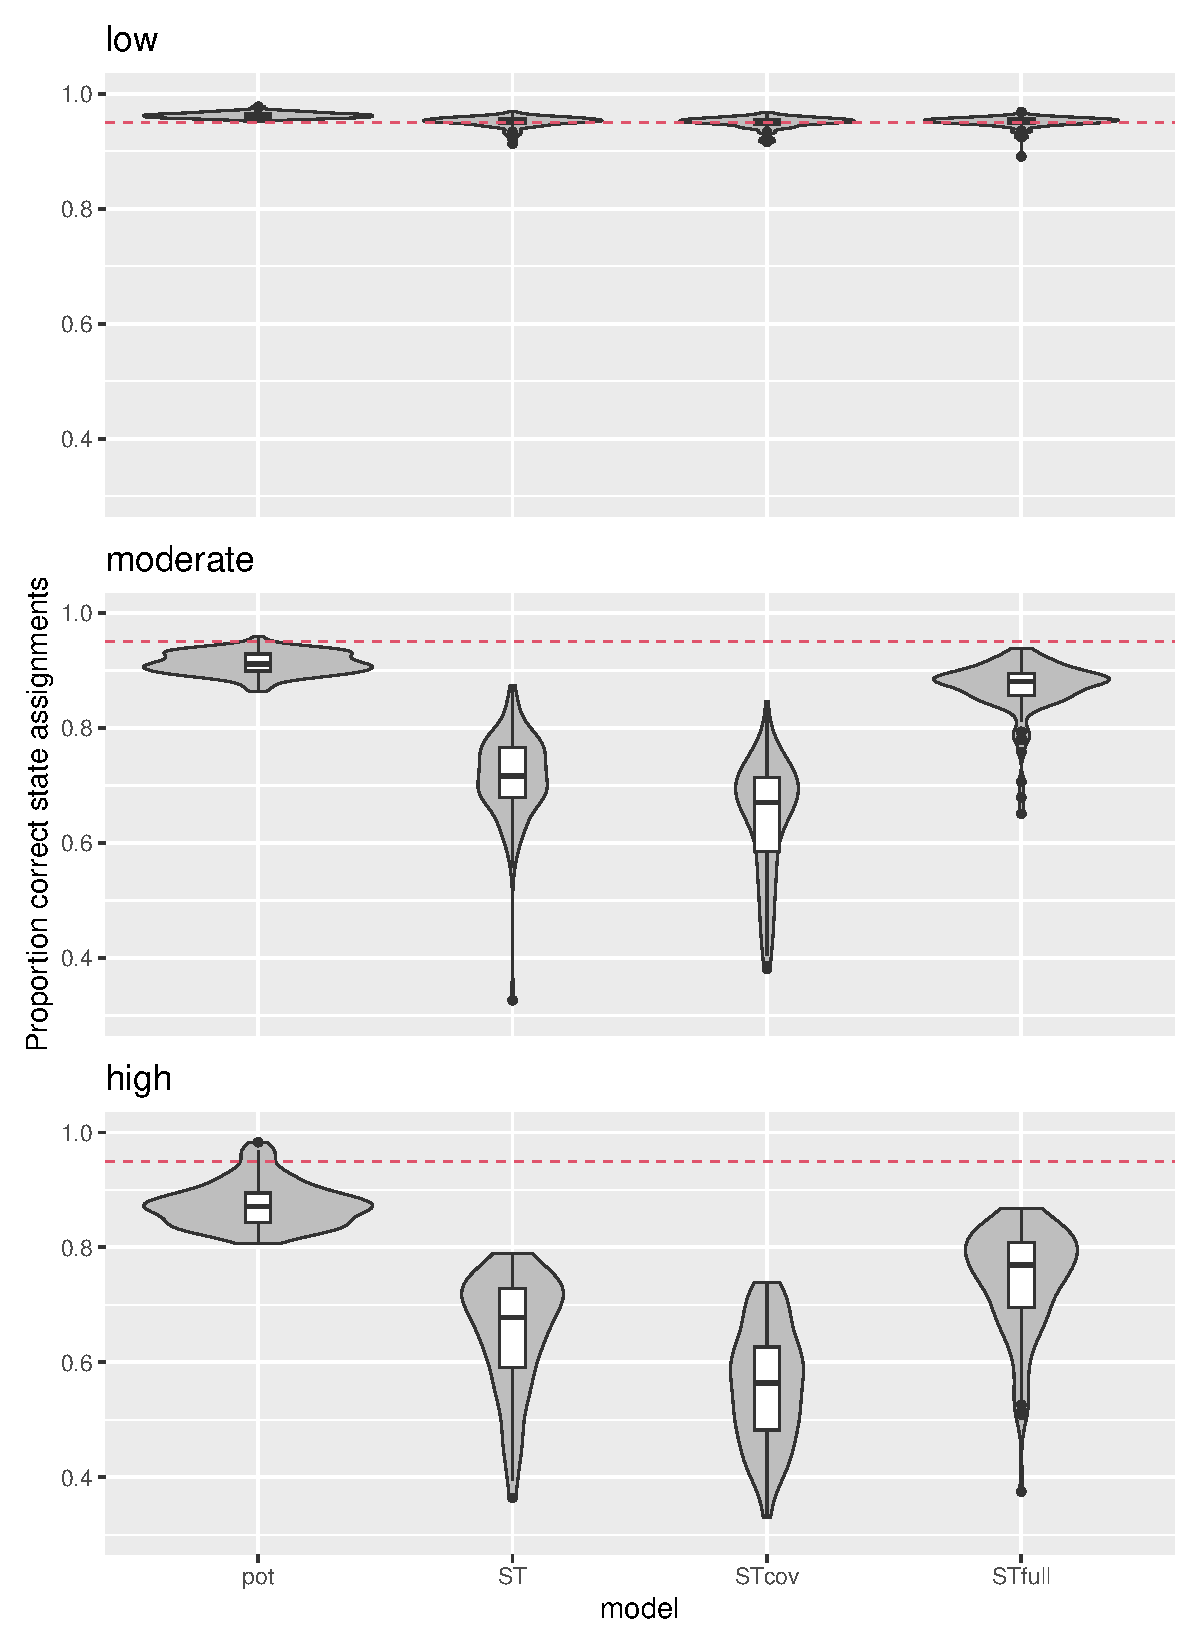
\includegraphics[width=0.9\textwidth]{../simulations/spat_noLangevinViterbiPlots.pdf}
    \caption{Violin plots for the proportion of correct Viterbi-decoded state assignments from simulations with data generated from a 2-state potential function HMM, with three degrees of overlap in the state-dependent observation distributions: ``low'' (top row), ``moderate'' (middle row), and ``high'' (bottom row). Four models were fitted to each simulated dataset: 1) the data-generating model (``pot''); 2) the standard 2-state step and turn HMM (``ST''); 3) a 2-state step and turn HMM including the habitat covariates on the observation distribution parameters (``STcov''); and 4) a 2-state step and turn HMM including transformed gradient-based habitat covariates on the observation distribution parameters.}
    \label{fig:spat_noLangevinViterbiPlots}
\end{figure}

\begin{figure}
    \centering
    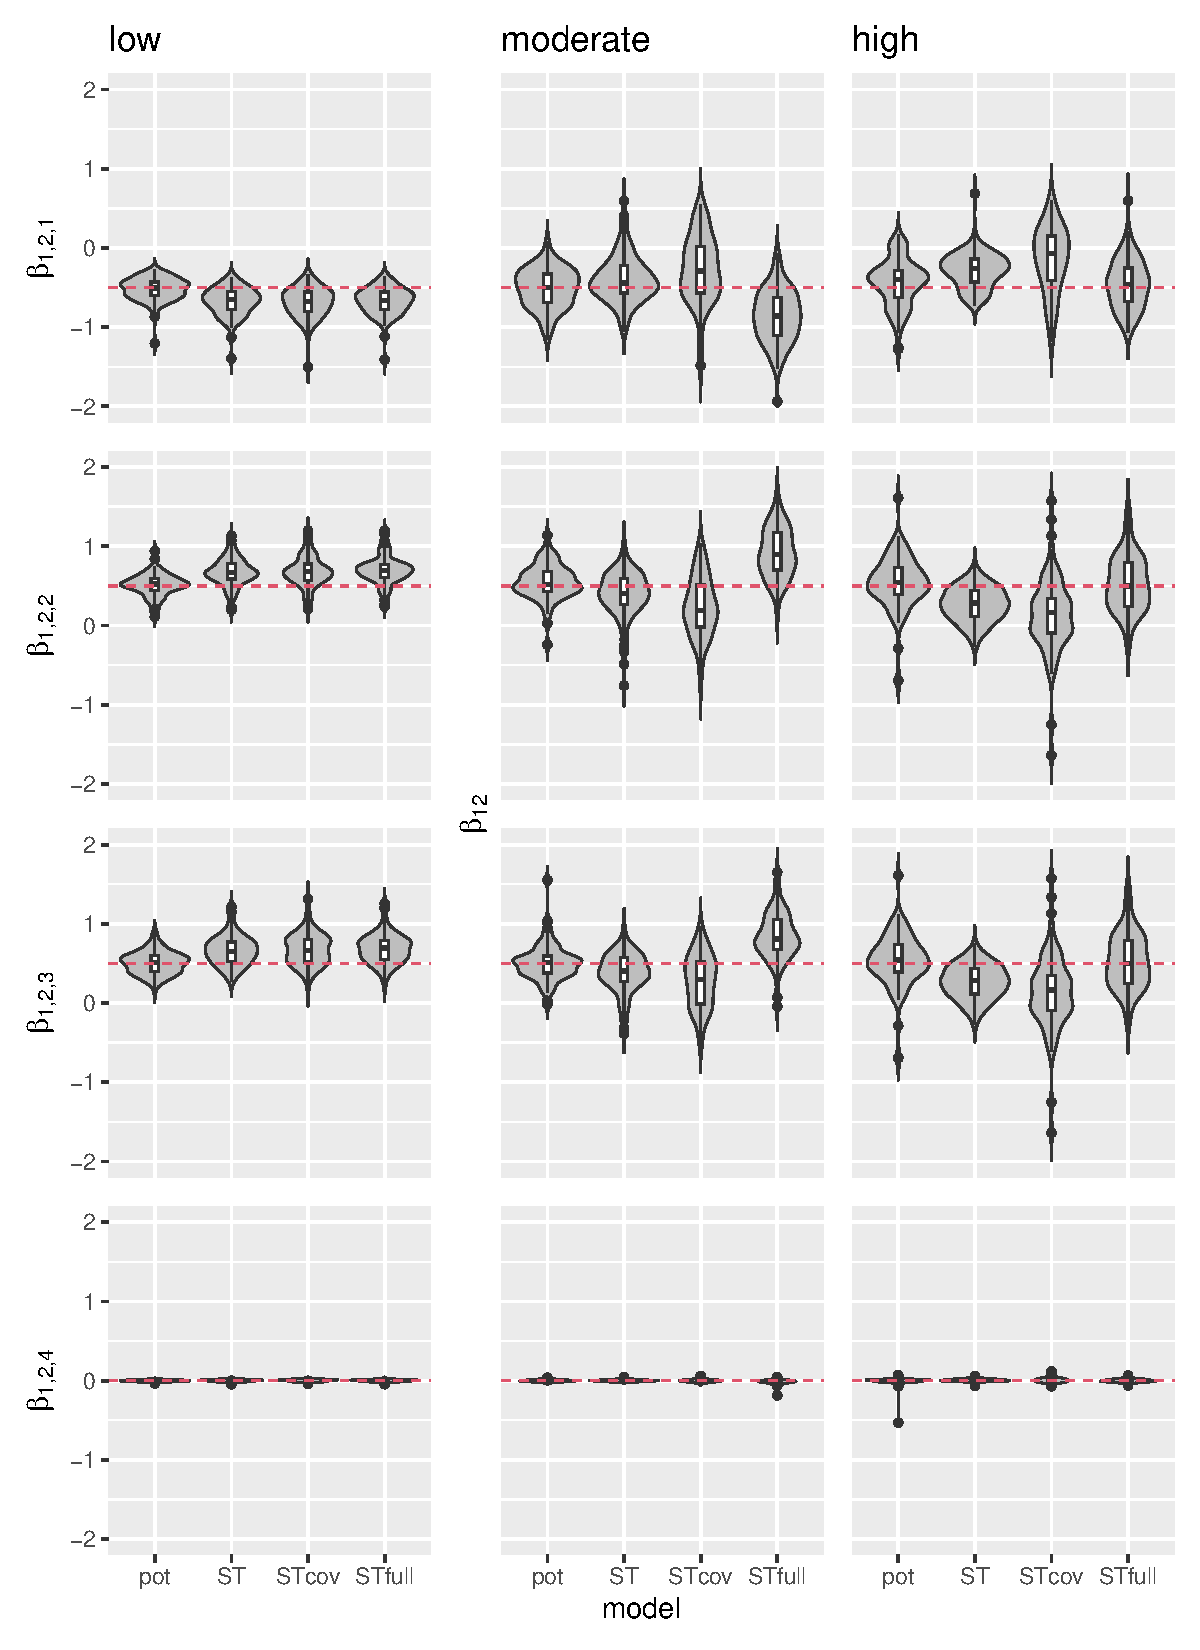
\includegraphics[width=0.8\textwidth]{../simulations/spat_noLangevinBeta12Plots.pdf}
    \caption{Violin plots for the estimated environmental covariate effects on transitions from state 2 to state 1 $\left(\beta_{1,2,k};k=1,\ldots,4\right)$ from 100 simulations with data generated from a 2-state potential function HMM, with three degrees of overlap in the state-dependent observation distributions: ``low'' (top row), ``moderate'' (middle row), and ``high'' (bottom row). 
    Four models were fitted to each simulated dataset: 1) the data-generating model (``pot''); 2) the standard 2-state step and turn HMM (``ST''); 3) a 2-state step and turn HMM including the habitat covariates on the observation distribution parameters (``STcov''); and 4) a 2-state step and turn HMM including transformed gradient-based habitat covariates on the observation distribution parameters.% For readability, the y-axis has been truncated at $(-1.75,1.75)$.
    }
    \label{fig:spat_noLangevinBeta12Plots}
\end{figure}

\begin{figure}
    \centering
    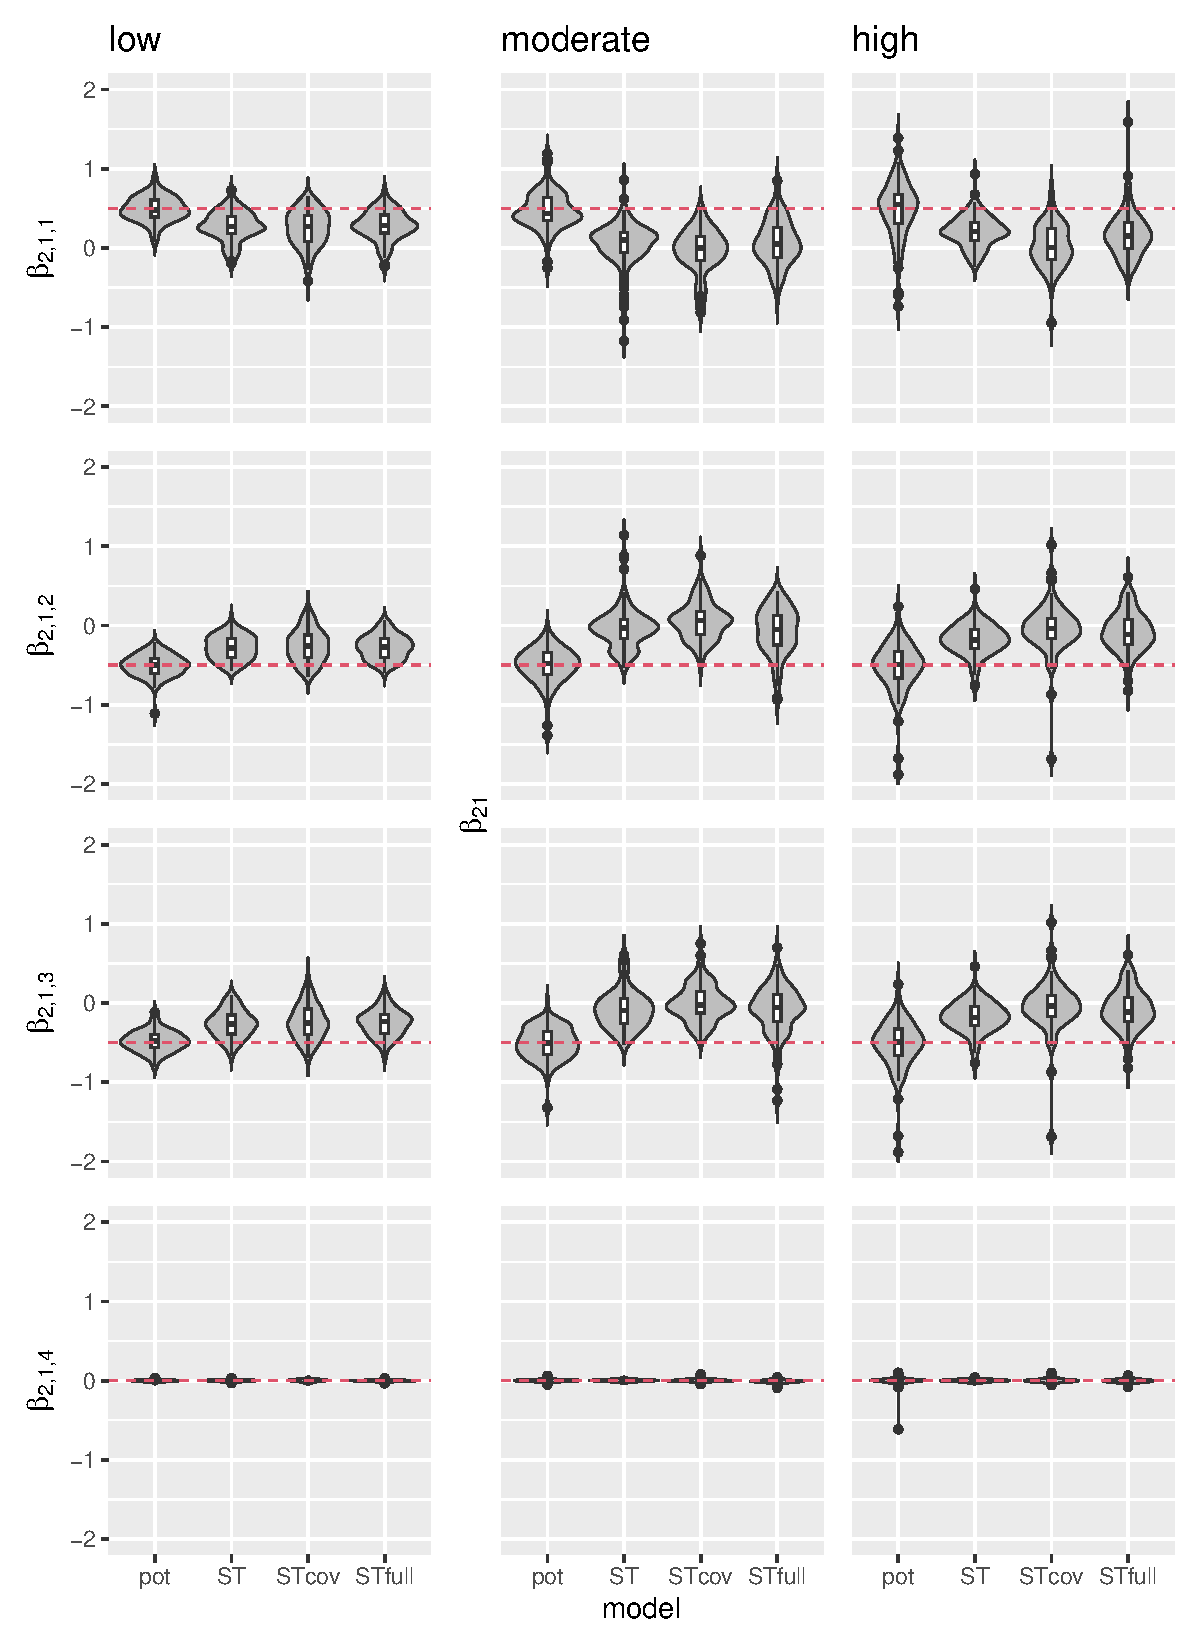
\includegraphics[width=0.8\textwidth]{../simulations/spat_noLangevinBeta21Plots.pdf}
    \caption{Violin plots for the estimated environmental covariate effects on transitions from state 2 to state 1 $\left(\beta_{2,1,k};k=1,\ldots,4\right)$ from 100 simulations with data generated from a 2-state potential function HMM, with three degrees of overlap in the state-dependent observation distributions: ``low'' (top row), ``moderate'' (middle row), and ``high'' (bottom row). 
    Four models were fitted to each simulated dataset: 1) the data-generating model (``pot''); 2) the standard 2-state step and turn HMM (``ST''); 3) a 2-state step and turn HMM including the habitat covariates on the observation distribution parameters (``STcov''); and 4) a 2-state step and turn HMM including transformed gradient-based habitat covariates on the observation distribution parameters.% For readability, the y-axis has been truncated at $(-1.75,1.75)$.
    }
    \label{fig:spat_noLangevinBeta21Plots}
\end{figure}

\begin{figure}
    \centering
    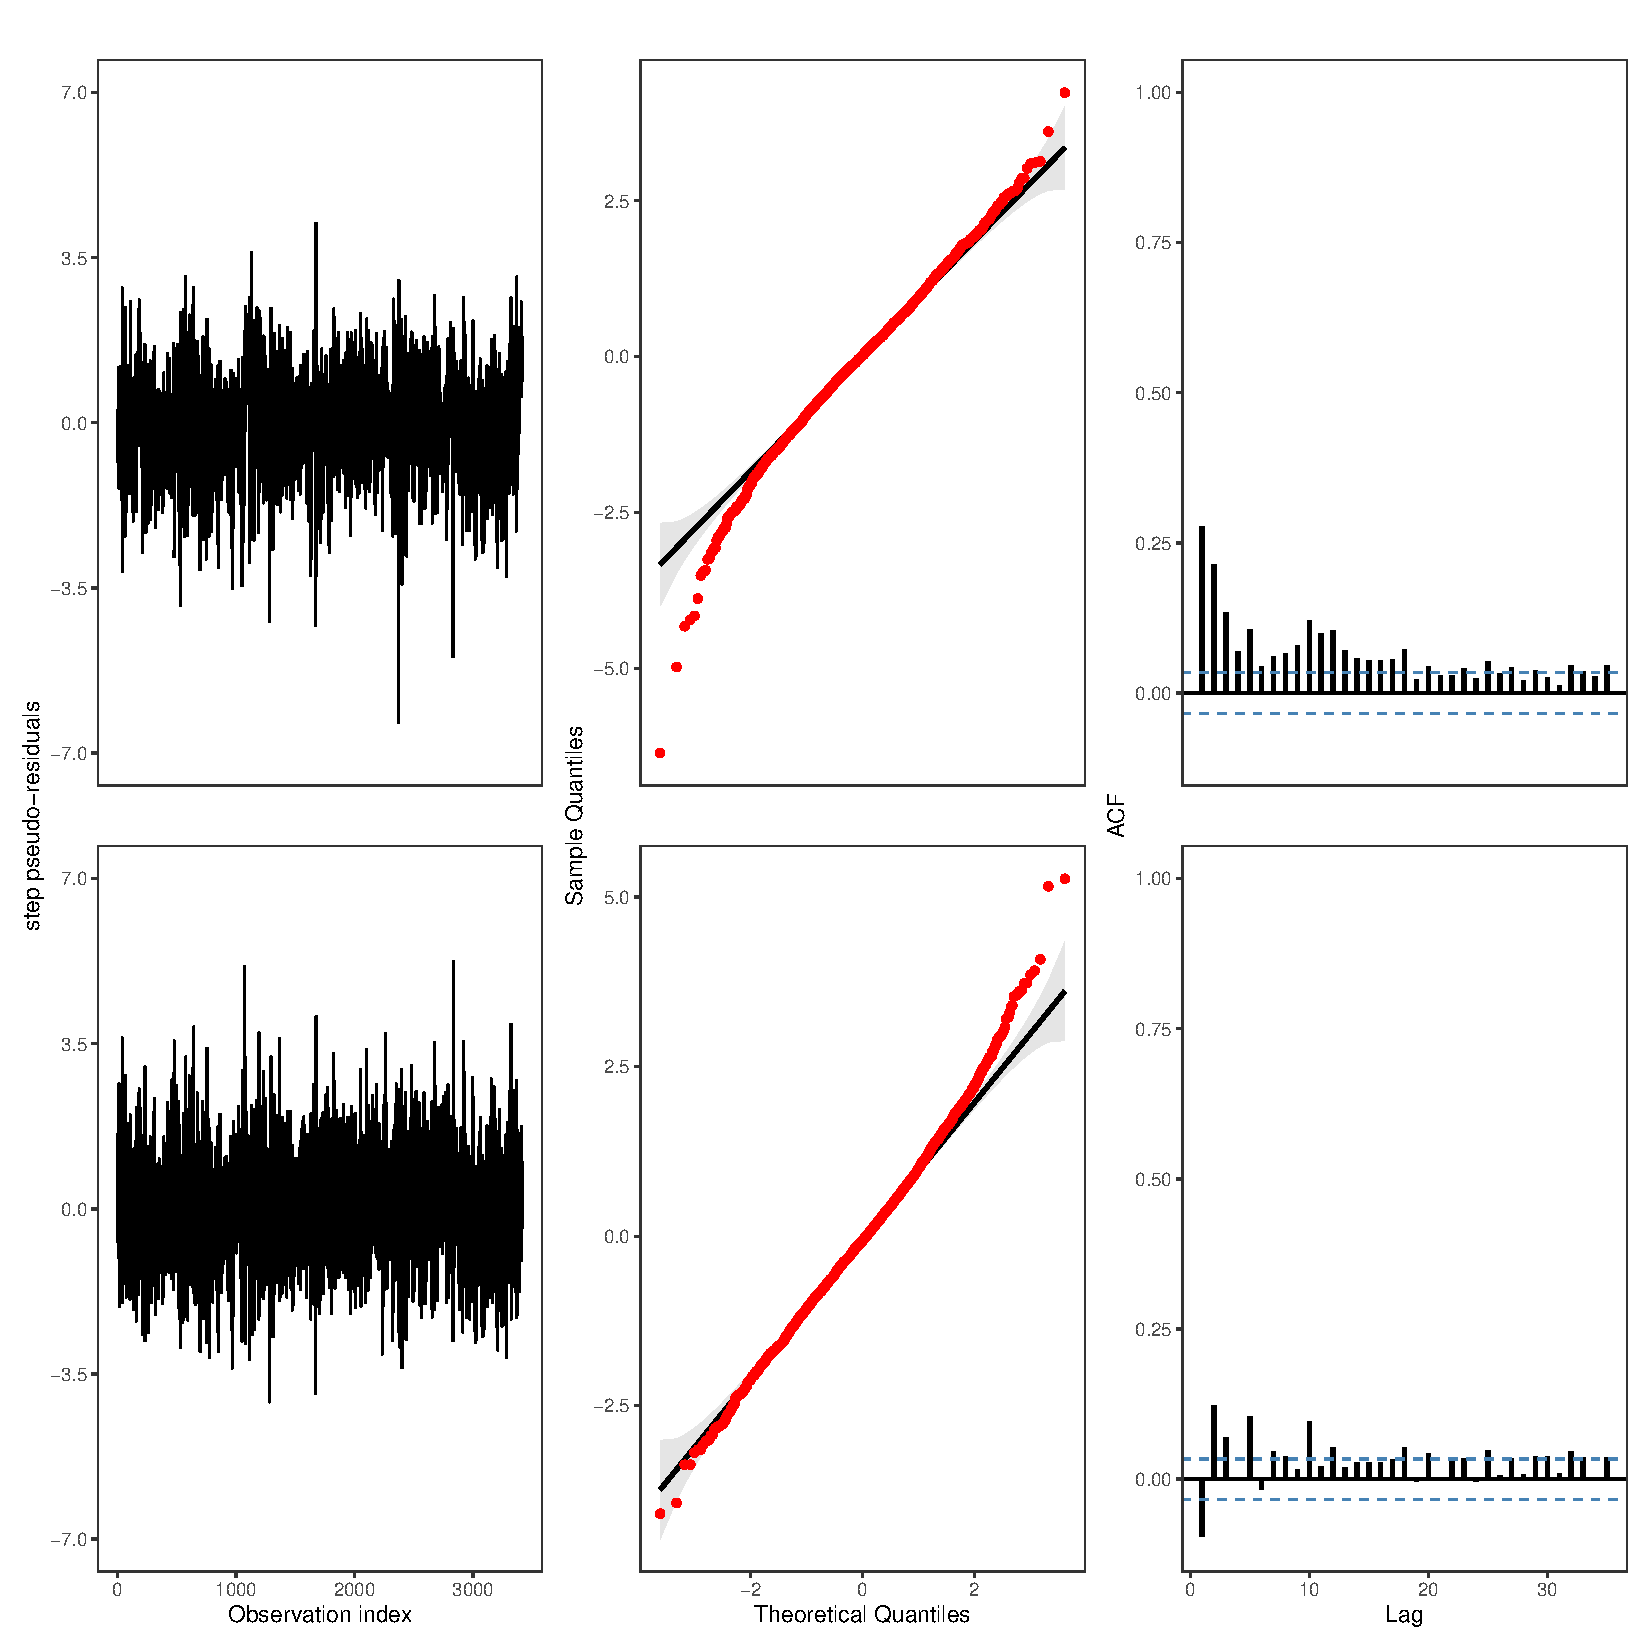
\includegraphics[width=0.9\textwidth]{../examples/ses/STsteppr.pdf}
    \caption{Step length pseudo-residual plots for the 4-state standard step and turn model (top row) and the correlated step and turn model (bottom row), including the raw pseudo-residual plot (left column), QQ plot (middle column), and autocorrelation function plot (ACF; right column).}
    \label{fig:STsteppr}
\end{figure}

\begin{figure}
    \centering
    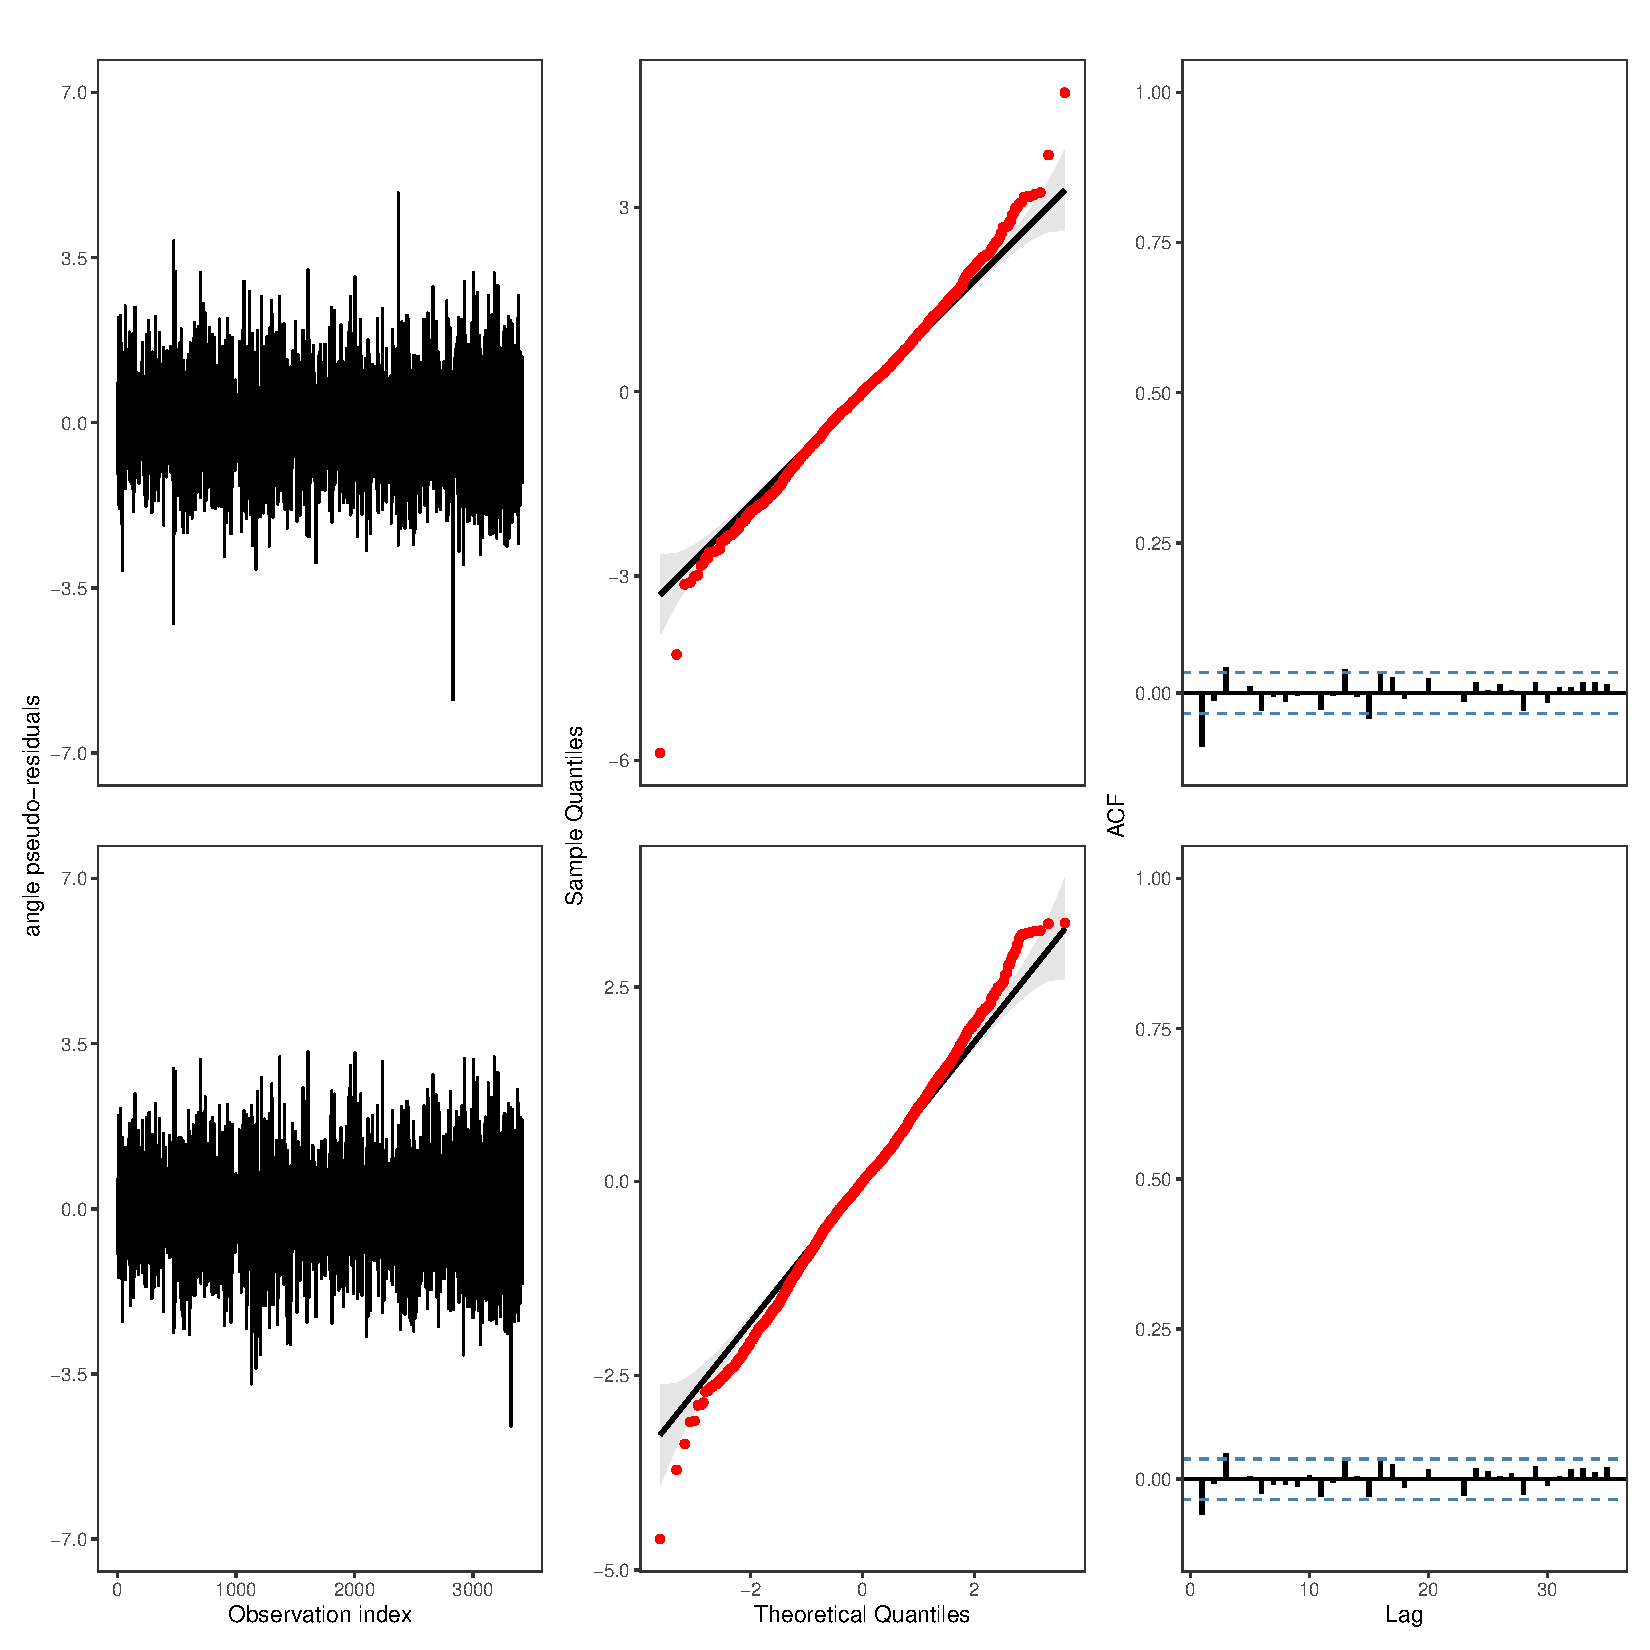
\includegraphics[width=0.9\textwidth]{../examples/ses/STanglepr.pdf}
    \caption{Turn angle pseudo-residual plots for the 4-state standard step and turn model (top row) and the correlated step and turn model (bottom row), including the raw pseudo-residual plot (left column), QQ plot (middle column), and autocorrelation function plot (ACF; right column).}
    \label{fig:STanglepr}
\end{figure}

\FloatBarrier

\begin{table}[h!]
\centering
\caption{Contingency table comparing the Viterbi-decoded state assignments for the 4-state standard step and turn model (``ST'') and the correlated step and turn model (``crwST'') in the southern elephant seal example.}
\label{tab:STstates}
\begin{tabular}{@{}lccccc@{}}
\toprule
& \multicolumn{5}{c}{\textbf{crwST}} \\
\cmidrule(l){2-6}
\textbf{ST} & \text{``outbound''} & \text{state 2} & \text{state 3} & \text{``inbound''} & \text{Total} \\
\midrule
\text{``outbound''} & 419 & 4   & 0   & 0  & 423 \\
\text{state 2} & 106 & 803 & 15   & 9 & 933 \\
\text{state 3} & 99  & 417 & 1140 & 5 & 1661  \\
\text{``inbound''} & 0   & 96   & 0   & 303 & 399 \\
\text{Total} & 624 & 1320 & 1155 & 317 & \\
\bottomrule
\end{tabular}
\end{table}

\begin{figure}
    \centering
    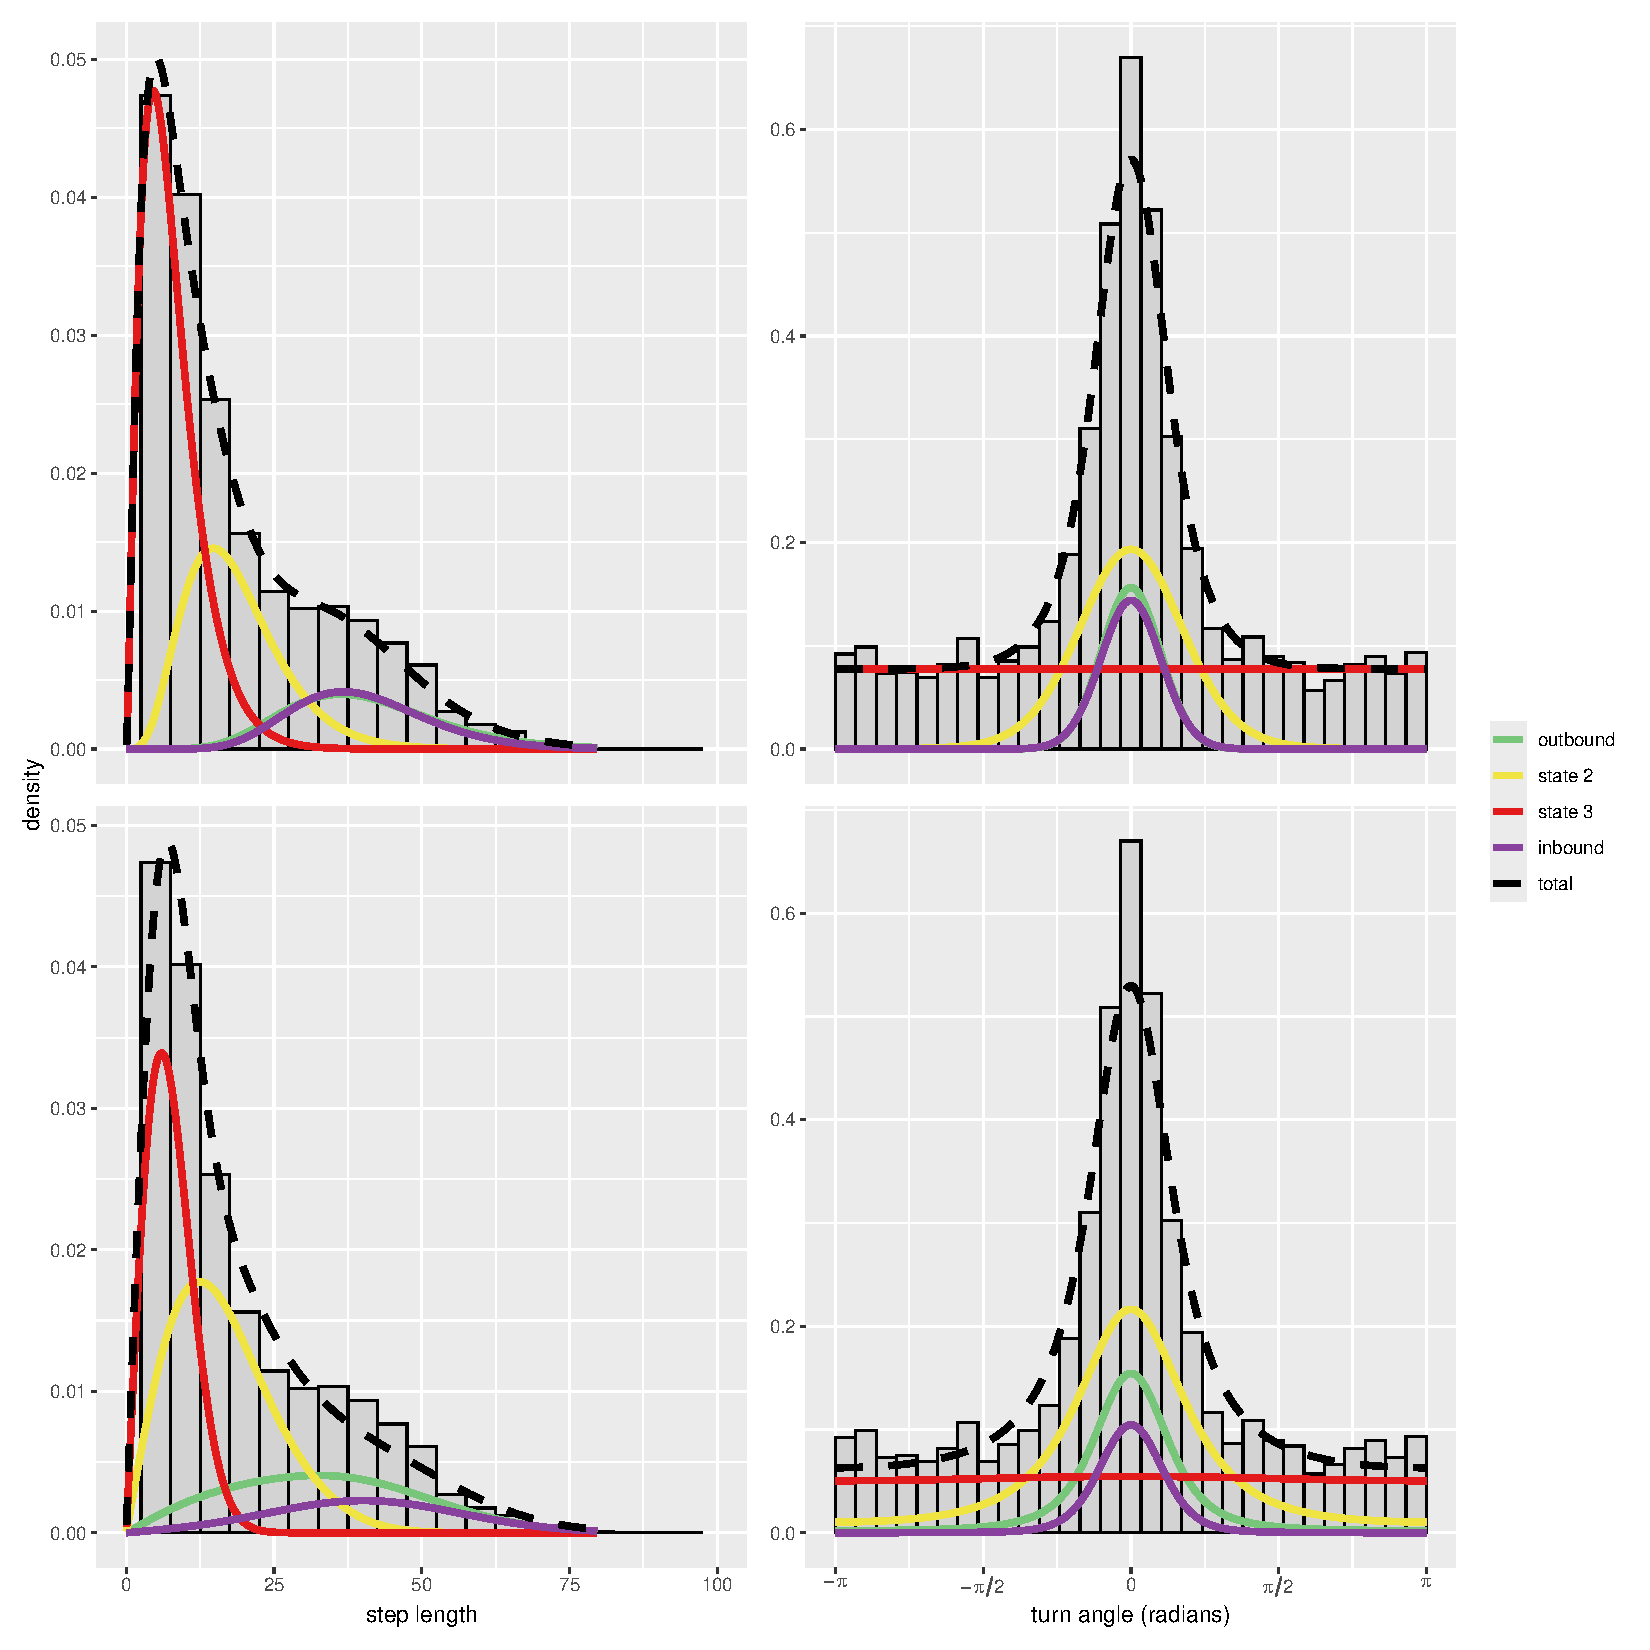
\includegraphics[width=0.9\textwidth]{../examples/ses/STdens.pdf}
    \caption{Estimated state-dependent distributions for step length (left column) and turn angle (right column) from the 4-state standard step and turn model (top row) and correlated step and turn model (bottom row) in the southern elephant seal example. Densities are weighted by the proportion of time steps assigned to each state based on the Viterbi algorithm.}
    \label{fig:STdens}
\end{figure}

\begin{figure}
    \centering
    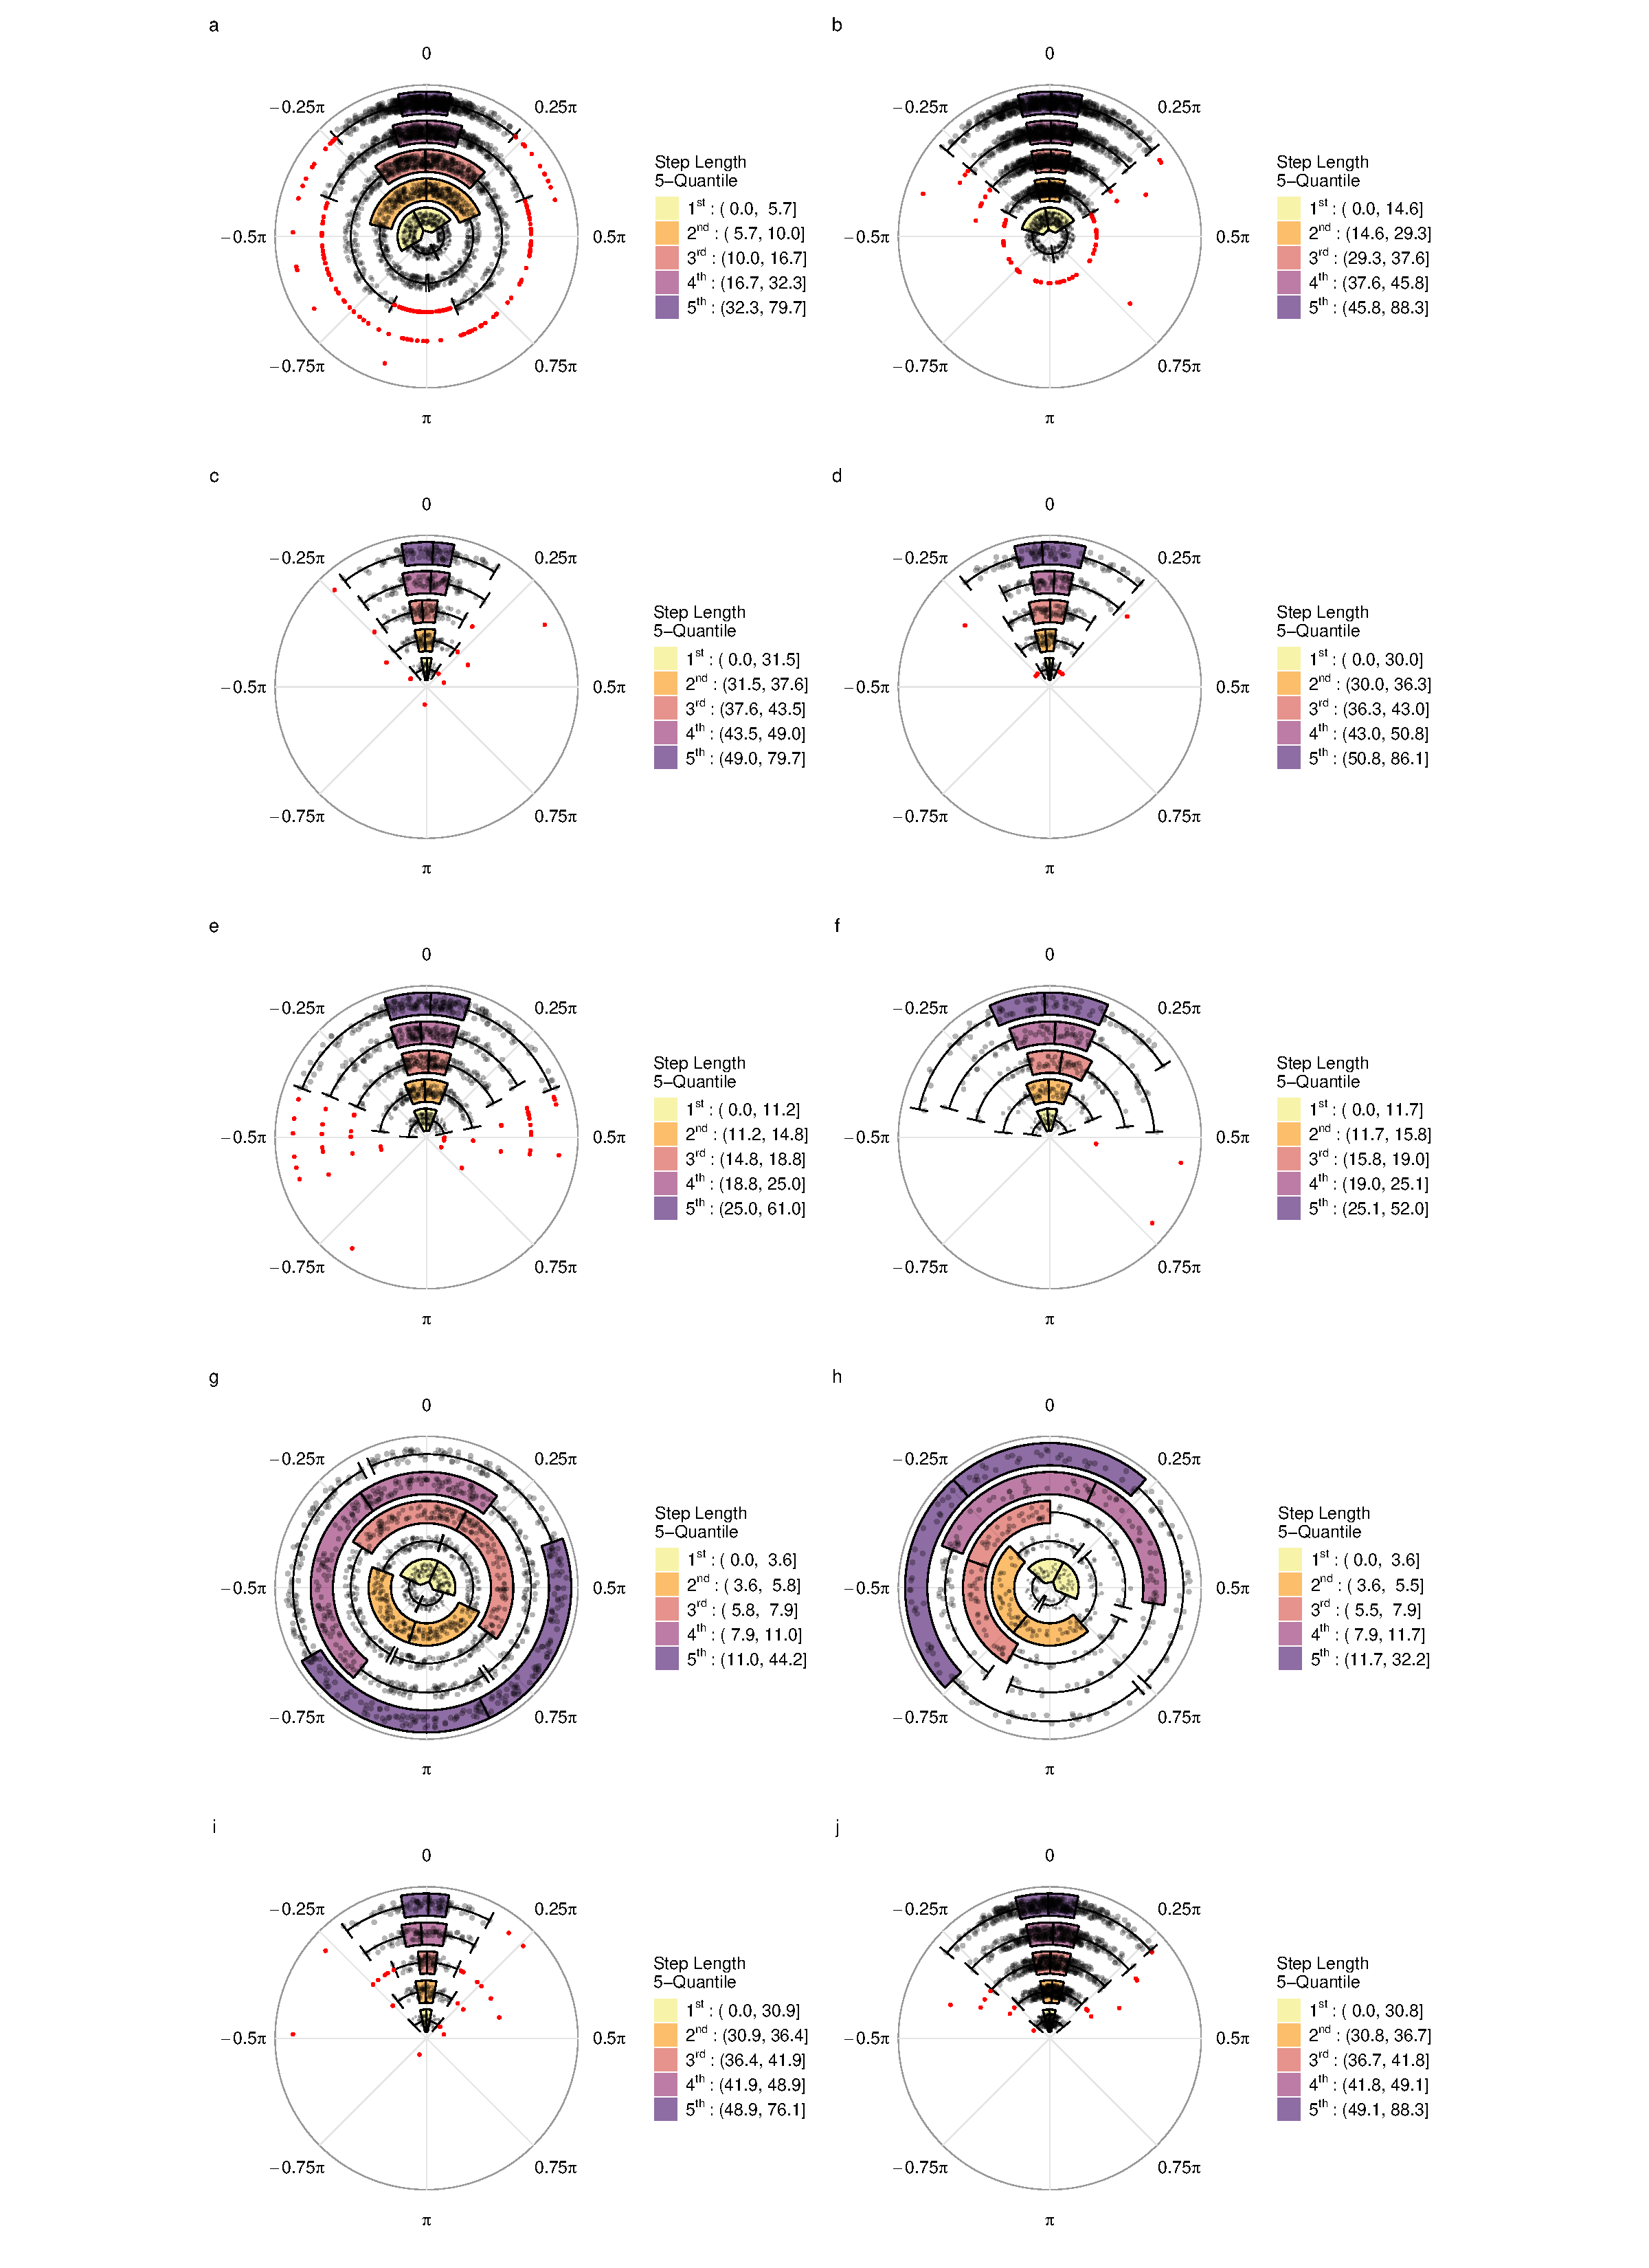
\includegraphics[width=0.9\textwidth]{../examples/ses/m1_cor.pdf}
    \caption{Circular box plots of the step lengths (km) and turn angles for the southern elephant seal data (left column) and data simulated from the fitted 4-state standard step and turn model (right column), where the top row includes all time steps and rows 2--5 correspond to time steps assigned to states 1--4, respectively. For each of the five step length quantiles, a box plot of the corresponding angles is shown. Outliers (i.e., values outside 1.5 times the inter quartile range) are marked in red. Top plot includes the data for all six individuals, and the bottom six plots correspond to each individual. Plots created using R package cylcop \citep{hodel2022circular}.}
    \label{fig:m1_cor}
\end{figure}

\begin{figure}
    \centering
    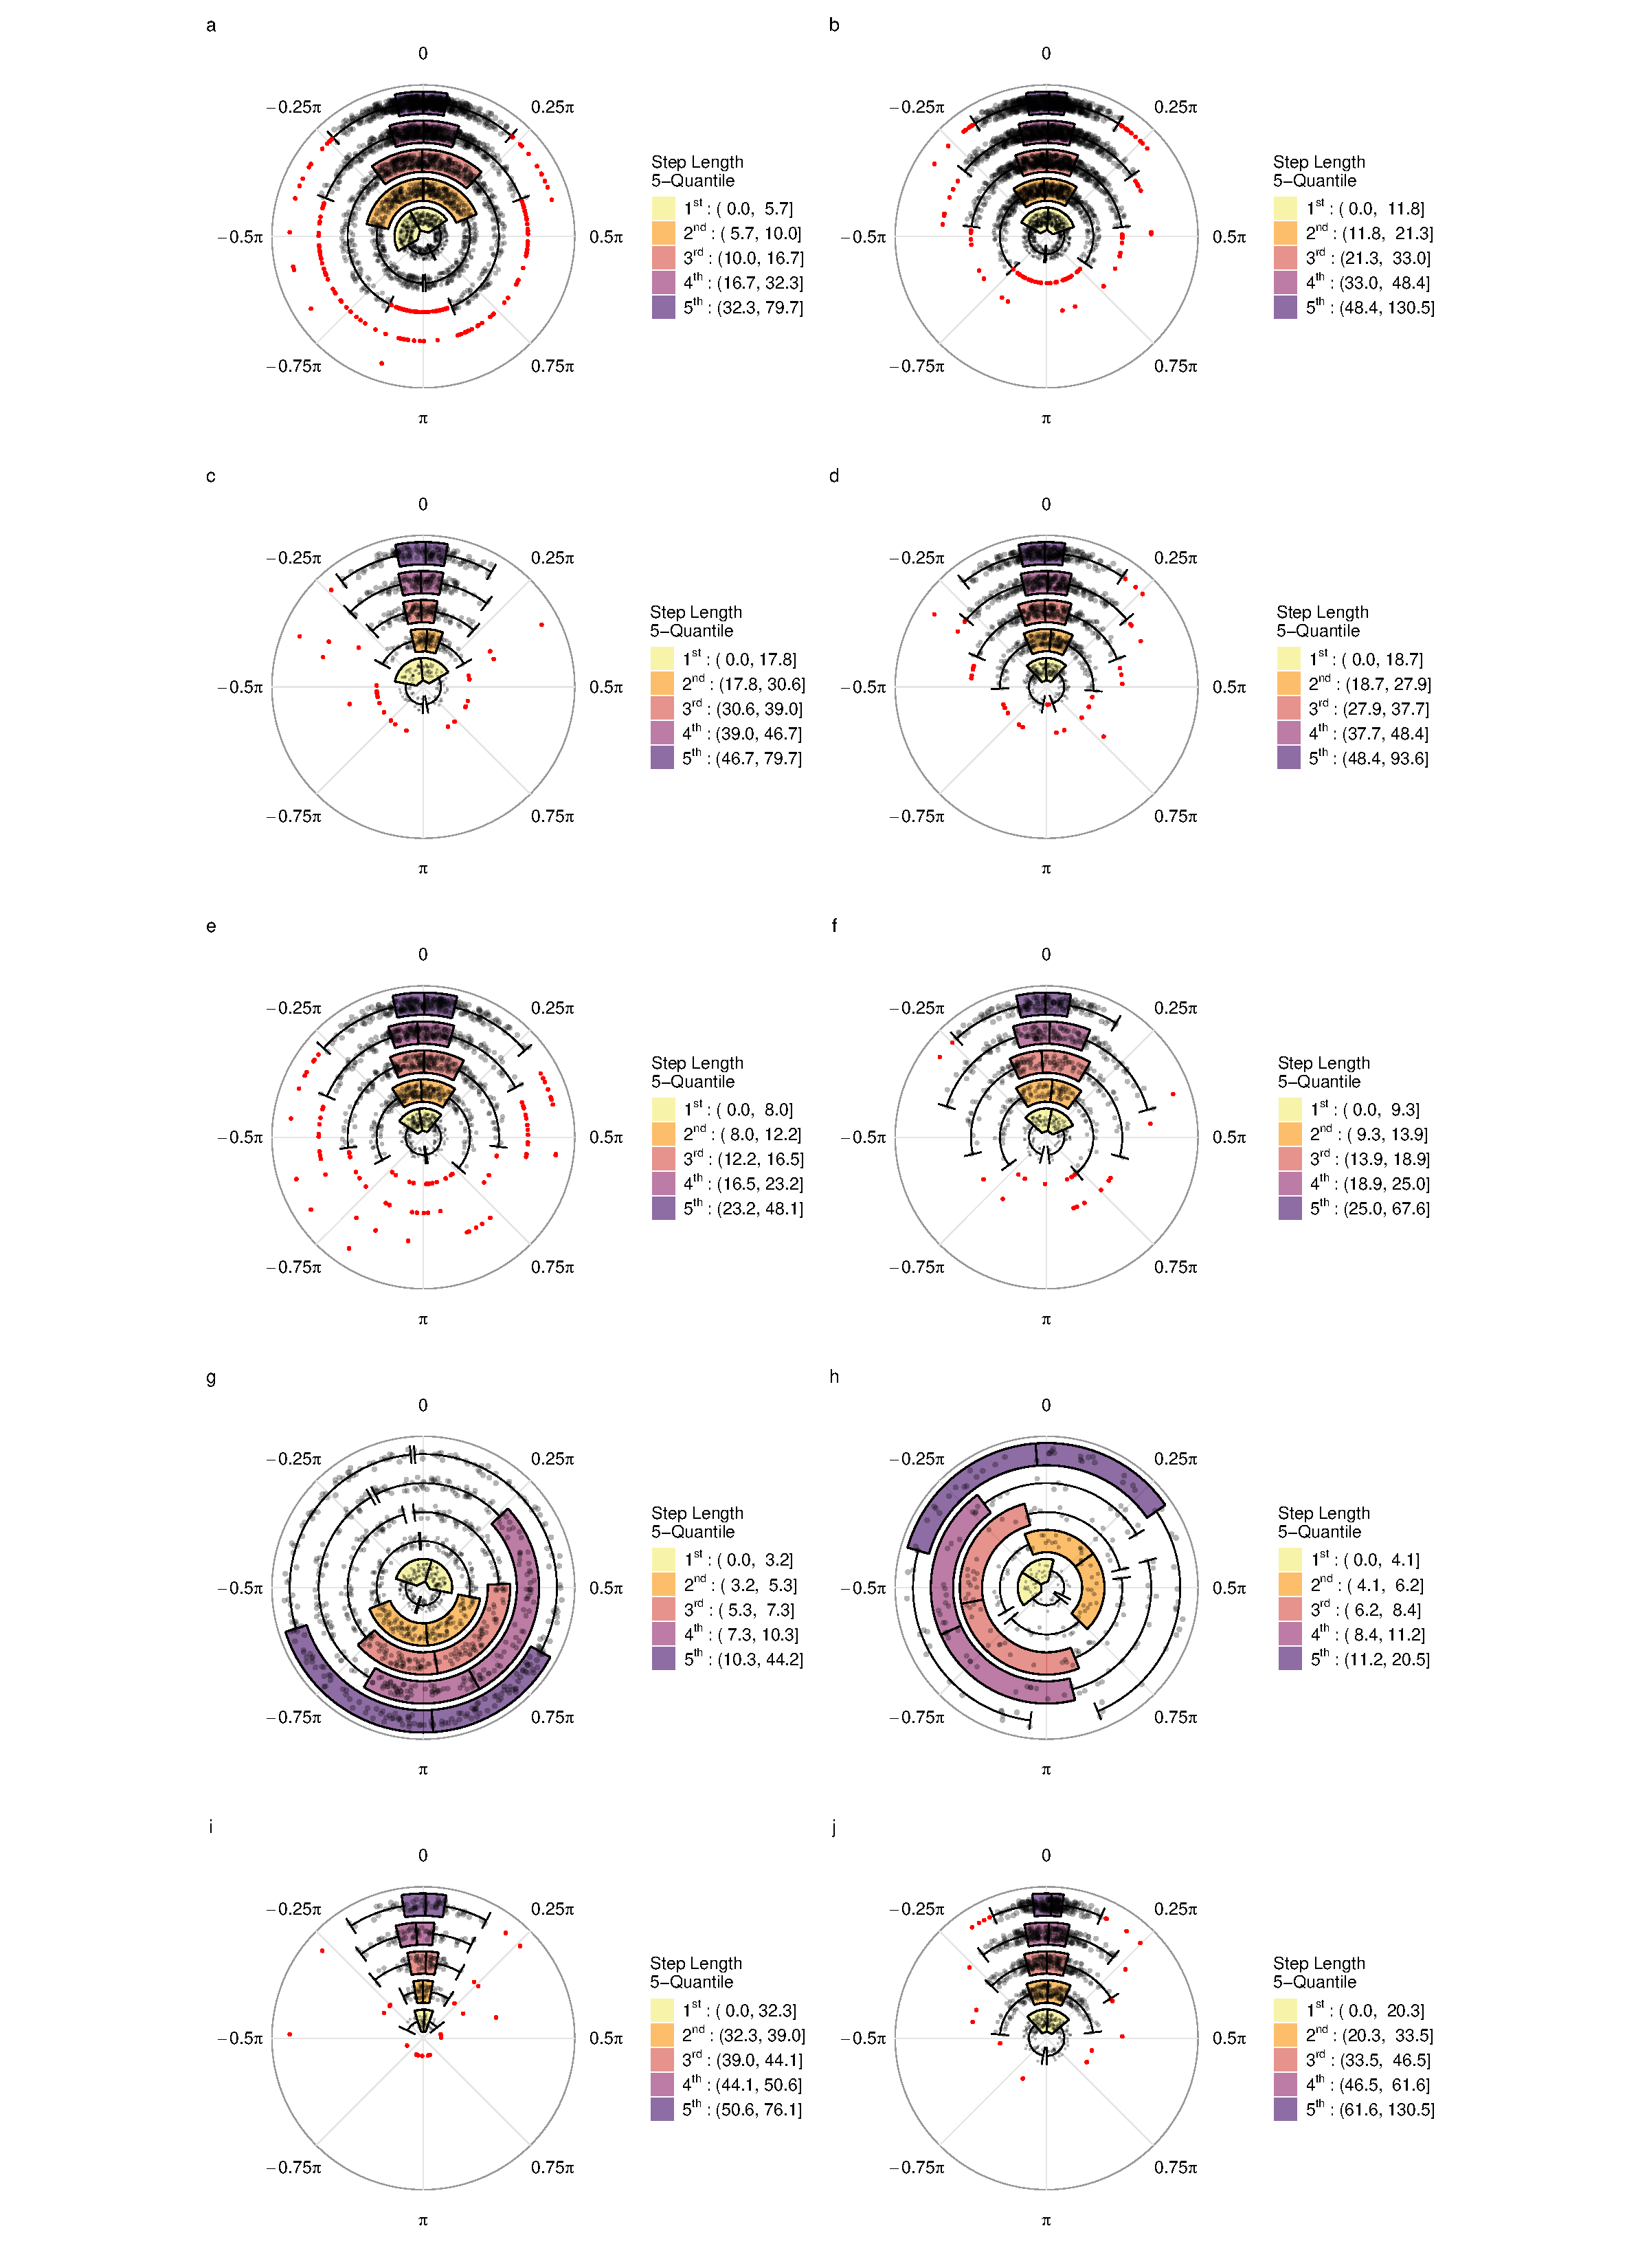
\includegraphics[width=0.9\textwidth]{../examples/ses/crwm1_cor.pdf}
    \caption{Circular box plots of the step lengths (km) and turn angles for the southern elephant seal data (left column) and data simulated from the fitted 4-state correlated step and turn model (right column), where the top row includes all time steps and rows 2--5 correspond to time steps assigned to states 1--4, respectively. For each of the five step length quantiles, a box plot of the corresponding angles is shown. Outliers (i.e., values outside 1.5 times the inter quartile range) are marked in red. Top plot includes the data for all six individuals, and the bottom six plots correspond to each individual. Plots created using R package cylcop \citep{hodel2022circular}.}
    \label{fig:crwm1_cor}
\end{figure}

\begin{figure}
    \centering
    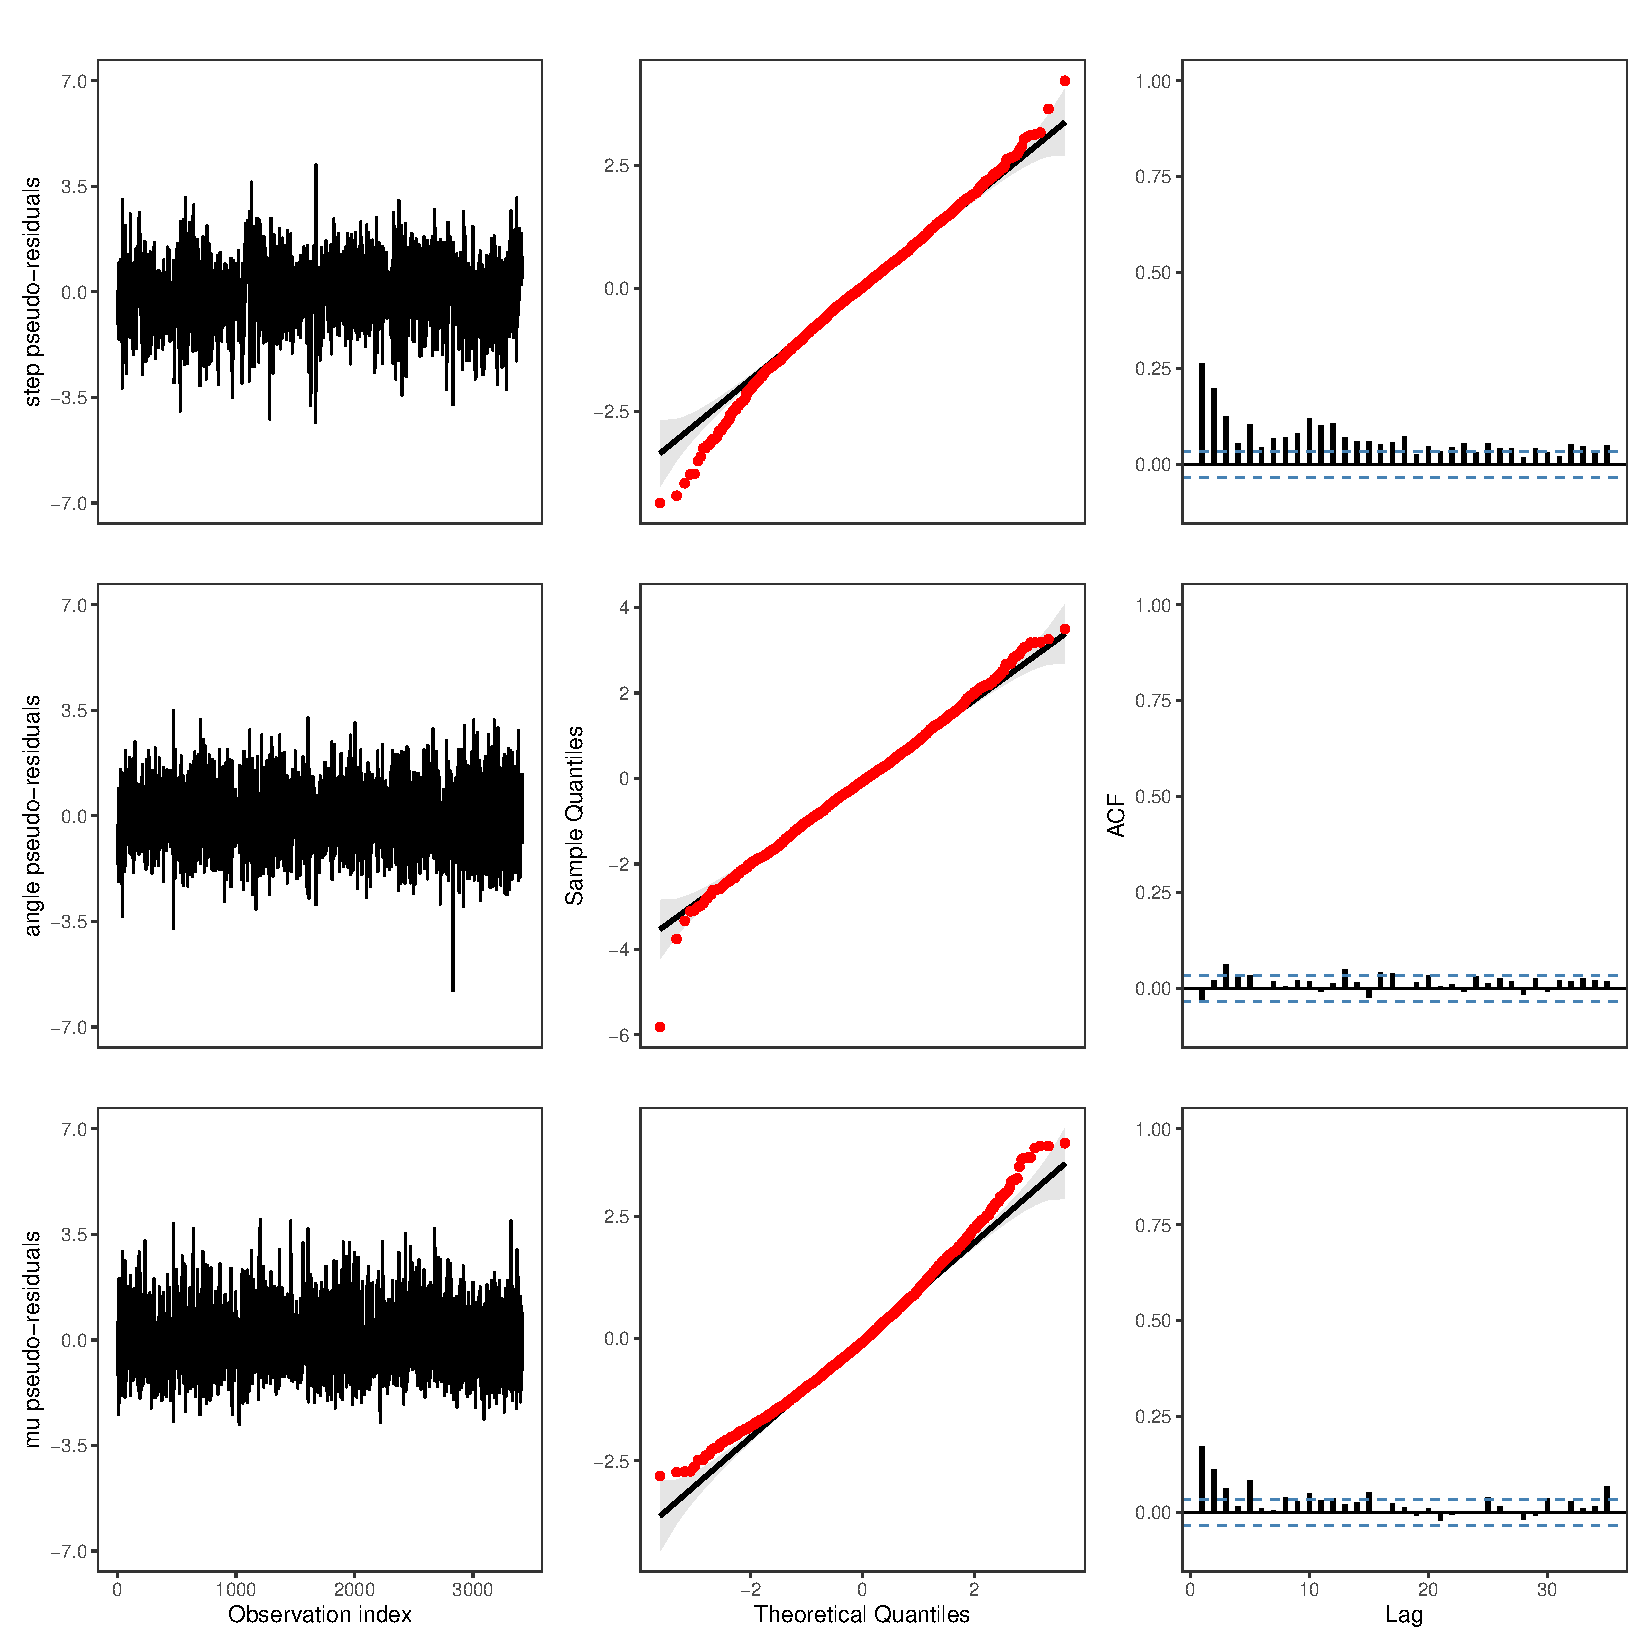
\includegraphics[width=0.9\textwidth]{../examples/ses/bcrwpr.pdf}
    \caption{Southern elephant seal step length (top row) and turn angle (middle row) pseudo-residual plots for the 4-state biased polar-based model, and location (``mu''; bottom row) pseudo-residual plots for the position-based potential function model. Diagnostics include the raw pseudo-residual plot (left column), QQ plot (middle column), and autocorrelation function plot (ACF; right column).}
    \label{fig:bcrwpr}
\end{figure}

\begin{figure}
    \centering
    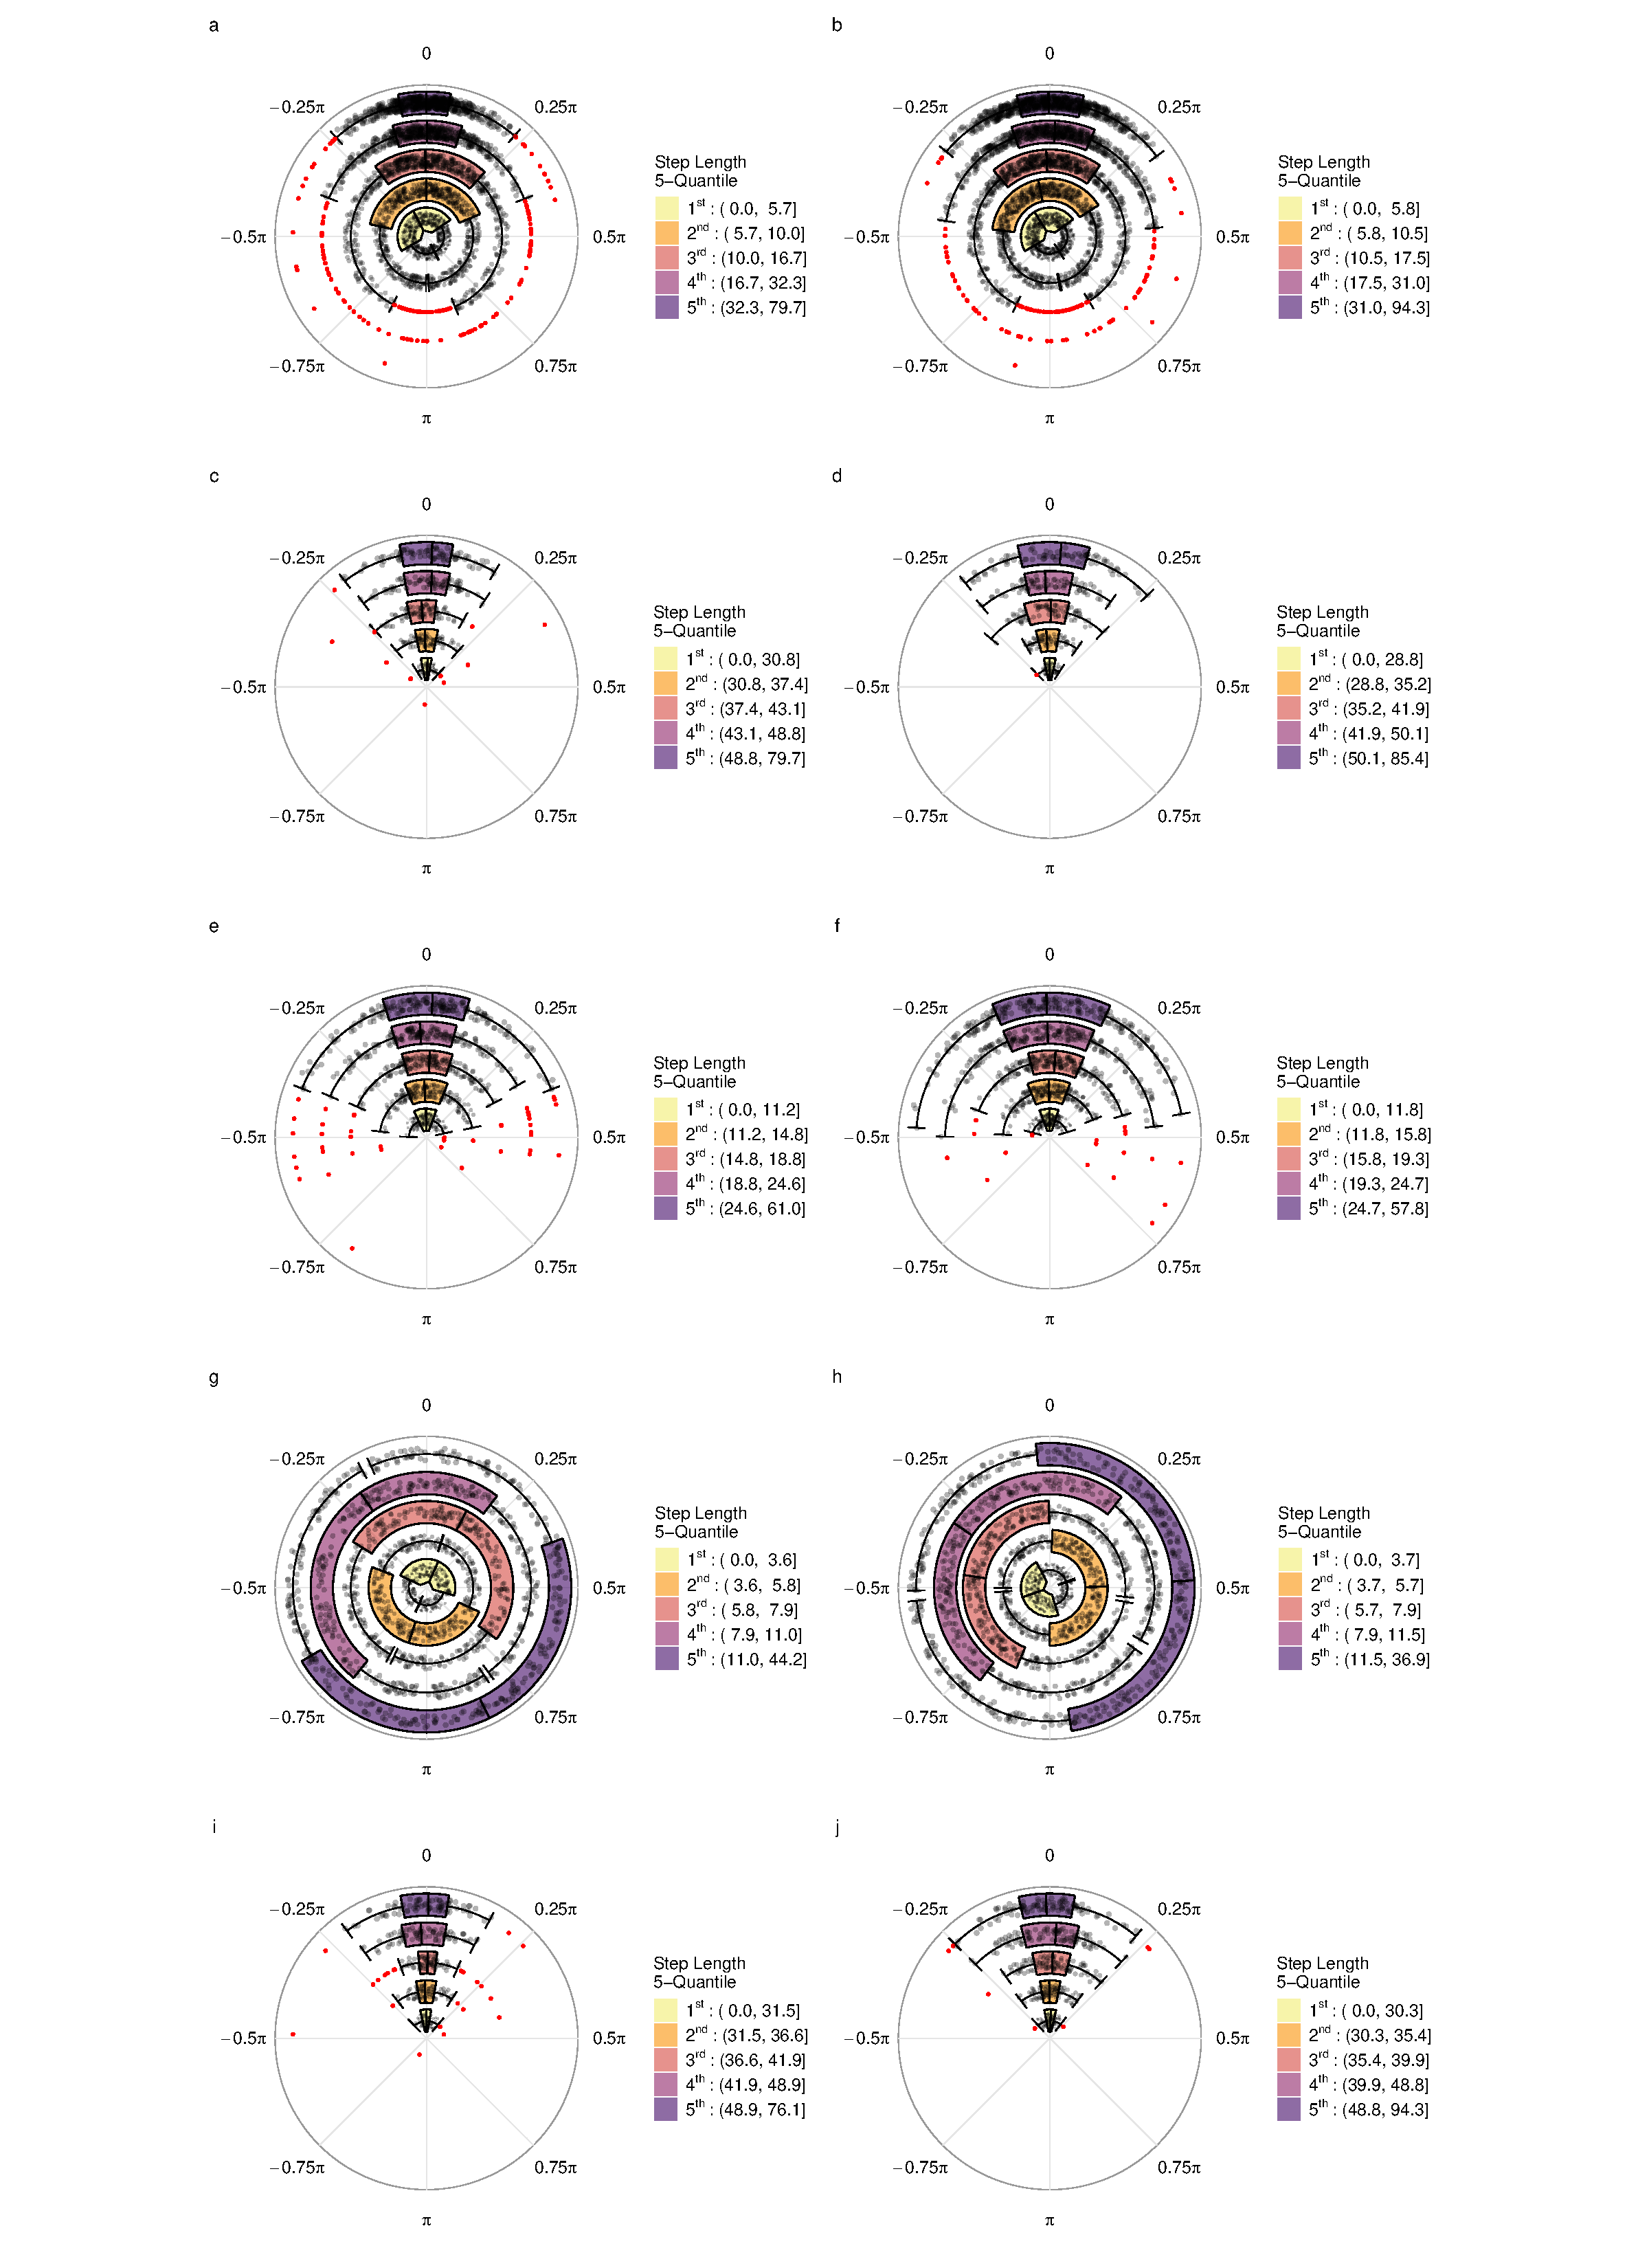
\includegraphics[width=0.9\textwidth]{../examples/ses/m2_cor.pdf}
    \caption{Circular box plots of the step lengths (km) and turn angles for the southern elephant seal data (left column) and data simulated from the fitted 4-state biased random walk step and turn model (right column), where the top row includes all time steps and rows 2--5 correspond to time steps assigned to states 1--4, respectively. For each of the five step length quantiles, a box plot of the corresponding angles is shown. Outliers (i.e., values outside 1.5 times the inter quartile range) are marked in red. Top plot includes the data for all six individuals, and the bottom six plots correspond to each individual. Plots created using R package cylcop \citep{hodel2022circular}.}
    \label{fig:m2_cor}
\end{figure}

\begin{figure}
    \centering
    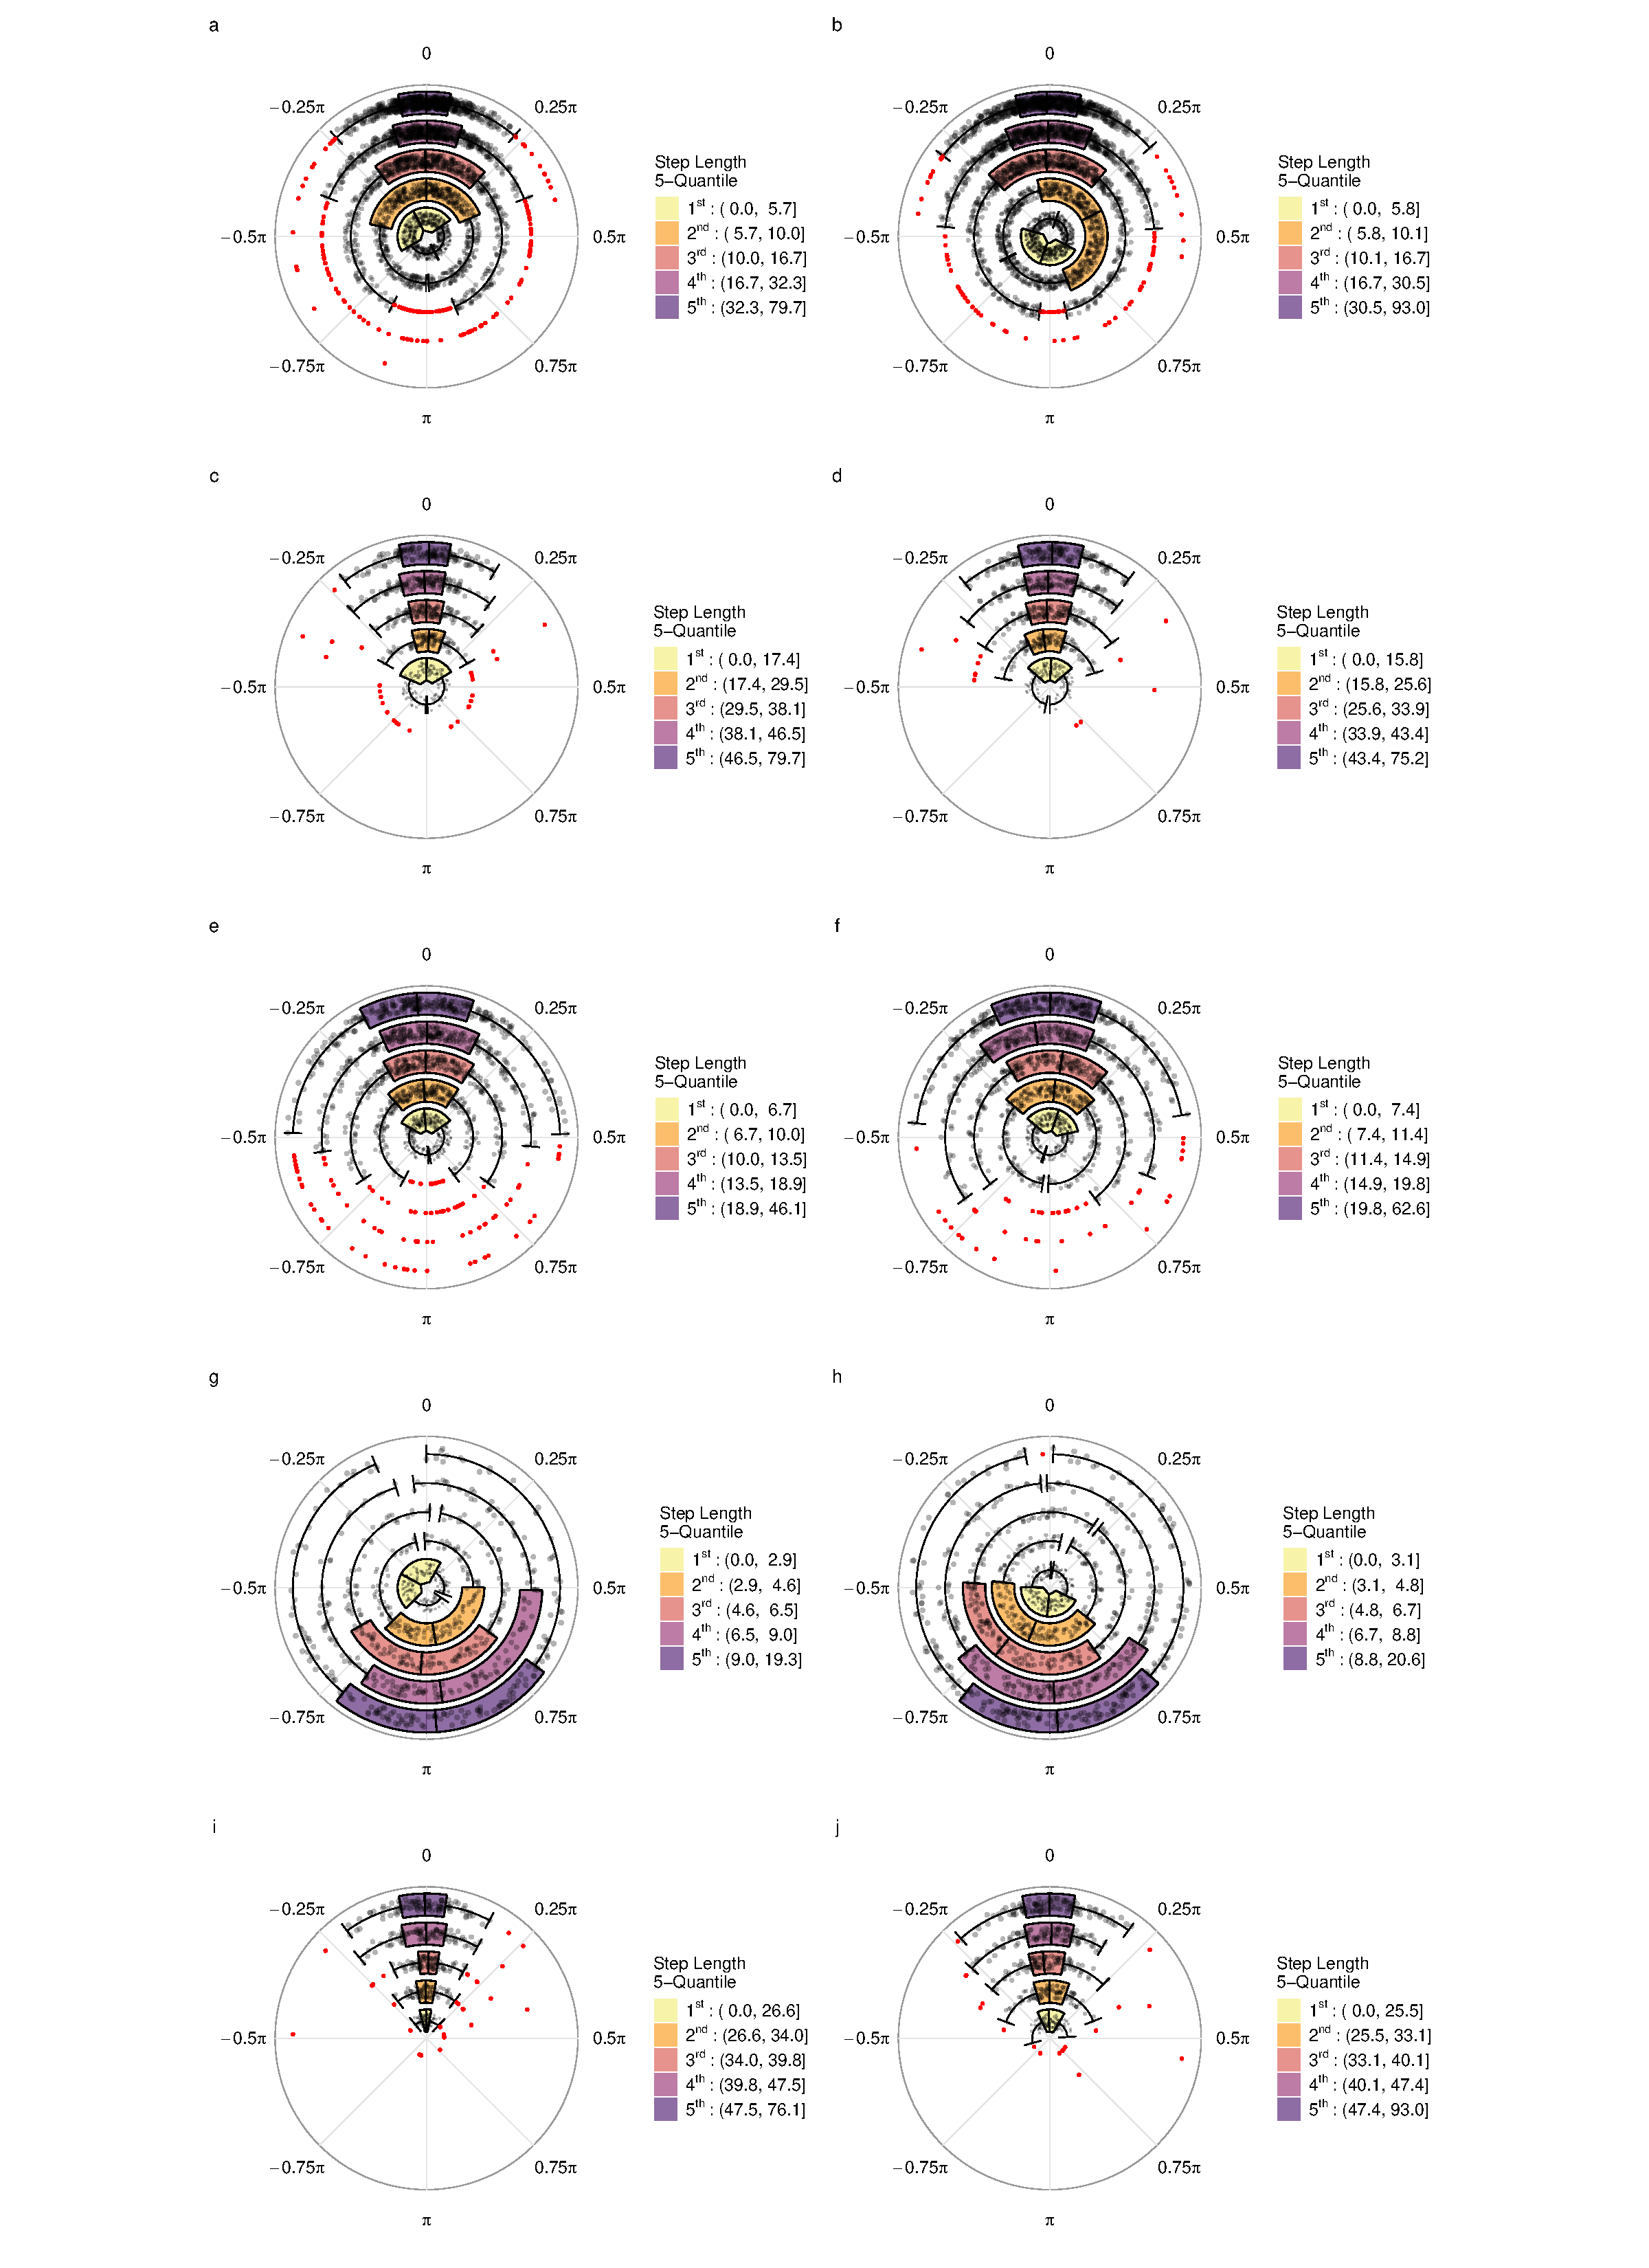
\includegraphics[width=0.9\textwidth]{../examples/ses/mpos_cor.pdf}
    \caption{Circular box plots of the step lengths (km) and turn angles for the southern elephant seal data (left column) and data simulated from the fitted 4-state position-based potential function model (right column), where the top row includes all time steps and rows 2--5 correspond to time steps assigned to states 1--4, respectively. For each of the five step length quantiles, a box plot of the corresponding angles is shown. Outliers (i.e., values outside 1.5 times the inter quartile range) are marked in red. Top plot includes the data for all six individuals, and the bottom six plots correspond to each individual. Plots created using R package cylcop \citep{hodel2022circular}.}
    \label{fig:mpos_cor}
\end{figure}

\FloatBarrier

\begin{longtable}{@{}lrrrr@{}}
\caption{Southern elephant seal parameter estimates from the 4-state position-based potential function model. Parameters are on the real scale for the state-specific mean paramters ($\mu_{c,s}; c \in \{x,y\}, s \in \{1,2,3,4\}$), the log scale for the state-specific speed parameters ($\sigma_s$), and the logit scale for the state transition probability parameters ($\gamma_{ij}; i,j \in \{1,2,3,4\}$). For $\mu_{c,s}$, $\beta_{crw}$ is the lag 1 autocorrelation parameter and $\delta_k$ is the potential function coefficient for covariate $k$. For $\sigma_s$ and $\gamma_{ij}$, $\beta_0$ is the intercept term and $\beta_k$ is the coefficent for covariate $k$. Covariates included Euclidean distance to coast (``d2coast''), anisotropically-scaled Euclidean distance from colony (``dfrcol''), study area boundary (``bound''), Euclidean distance to colony (``d2col''), sea floor depth (``bath''), Euclidean distance inland (``land''), and time since departure from the colony (``time'').} \label{tab:model_params} \\

\toprule
Parameter & Est & SE & LCI & UCI \\
\bottomrule
$\mu_{x,1}$: $\beta_{crw}$ & 0.42 & 0.04 & 0.35 & 0.49 \\
$\mu_{x,1}$: $\delta_{d2coast}$ & -0.01 & 0.00 & -0.01 & -0.01 \\
$\mu_{x,1}$: $\delta_{dfrcol}$ & 0.25 & 0.02 & 0.21 & 0.29 \\
$\mu_{x,1}$: $\delta_{bound}$ & 1.53 & 0.23 & 1.07 & 1.98 \\
\hdashline
$\mu_{x,2}$: $\beta_{crw}$ & 0.67 & 0.02 & 0.62 & 0.71 \\
$\mu_{x,2}$: $\delta_{d2coast}$ & -0.00 & 0.00 & -0.00 & -0.00 \\
\hdashline
$\mu_{x,3}$: $\beta_{crw}$ & -0.34 & 0.03 & -0.41 & -0.27 \\
$\mu_{x,3}$: $\delta_{d2coast}$ & -0.00 & 0.00 & -0.00 & -0.00 \\
\hdashline
$\mu_{x,4}$: $\beta_{crw}$ & 0.66 & 0.03 & 0.59 & 0.72 \\
$\mu_{x,4}$: $\delta_{d2col}$ & -0.01 & 0.00 & -0.01 & -0.01 \\
\hdashline
$\mu_{y,1}$: $\beta_{crw}$ & 0.61 & 0.03 & 0.55 & 0.67 \\
$\mu_{y,1}$: $\delta_{d2coast}$ & -0.01 & 0.00 & -0.02 & -0.01 \\
$\mu_{y,1}$: $\delta_{dfrcol}$ & 0.00 & 0.00 & -0.00 & 0.00 \\
$\mu_{y,1}$: $\delta_{bound}$ & 0.41 & 0.60 & -0.76 & 1.59 \\
\hdashline
$\mu_{y,2}$: $\beta_{crw}$ & 0.66 & 0.03 & 0.61 & 0.71 \\
$\mu_{y,2}$: $\delta_{d2coast}$ & -0.00 & 0.00 & -0.00 & -0.00 \\
\hdashline
$\mu_{y,3}$: $\beta_{crw}$ & -0.16 & 0.04 & -0.24 & -0.09 \\
$\mu_{y,3}$: $\delta_{d2coast}$ & -0.00 & 0.00 & -0.00 & -0.00 \\
\hdashline
$\mu_{y,4}$: $\beta_{crw}$ & 0.61 & 0.05 & 0.51 & 0.70 \\
$\mu_{y,4}$: $\delta_{d2col}$ & -0.02 & 0.00 & -0.02 & -0.01 \\
\hdashline
$\sigma_{1}$: $\beta_0$ & -4.10 & 0.08 & -4.26 & -3.94 \\
$\sigma_{1}$: $\beta_{bath}$ & 0.05 & 0.01 & 0.03 & 0.08 \\
$\sigma_{1}$: $\beta_{d2coast}$ & -0.09 & 0.04 & -0.18 & -0.01 \\
$\sigma_{1}$: $\beta_{land}$ & 5.68 & 1.64 & 2.47 & 8.89 \\
$\sigma_{1}$: $\beta_{d2col}$ & -0.08 & 0.02 & -0.12 & -0.04 \\
\hdashline
$\sigma_{2}$: $\beta_0$ & -4.42 & 0.05 & -4.52 & -4.32 \\
$\sigma_{2}$: $\beta_{bath}$ & 0.13 & 0.02 & 0.10 & 0.17 \\
$\sigma_{2}$: $\beta_{d2coast}$ & 0.20 & 0.05 & 0.11 & 0.29 \\
$\sigma_{2}$: $\beta_{land}$ & 3.70 & 0.93 & 1.87 & 5.53 \\
\hdashline
$\sigma_{3}$: $\beta_0$ & -5.36 & 0.09 & -5.54 & -5.19 \\
$\sigma_{3}$: $\beta_{bath}$ & -0.07 & 0.03 & -0.12 & -0.02 \\
$\sigma_{3}$: $\beta_{d2coast}$ & -0.49 & 0.16 & -0.80 & -0.18 \\
$\sigma_{3}$: $\beta_{land}$ & 0.59 & 0.84 & -1.06 & 2.24 \\
\hdashline
$\sigma_{4}$: $\beta_0$ & -4.18 & 0.15 & -4.48 & -3.88 \\
$\sigma_{4}$: $\beta_{bath}$ & 0.08 & 0.03 & 0.03 & 0.13 \\
$\sigma_{4}$: $\beta_{d2coast}$ & 0.03 & 0.07 & -0.12 & 0.17 \\
$\sigma_{4}$: $\beta_{land}$ & 1.76 & 2.41 & -2.96 & 6.48 \\
$\sigma_{4}$: $\beta_{d2col}$ & -0.08 & 0.04 & -0.15 & -0.01 \\
\hdashline
$\gamma_{12}$: $\beta_0$ & -33.52 & 0.11 & -33.74 & -33.30 \\
$\gamma_{12}$: $\beta_{bath}$ & -0.90 & 0.45 & -1.78 & -0.02 \\
$\gamma_{12}$: $\beta_{d2col}$ & 50.44 & 0.19 & 50.07 & 50.80 \\
$\gamma_{12}$: $\beta_{d2col^2}$ & -18.68 & 0.22 & -19.11 & -18.26 \\
$\gamma_{12}$: $\beta_{d2col^3}$ & 2.24 & 0.07 & 2.10 & 2.37 \\
$\gamma_{12}$: $\beta_{d2coast}$ & -104.96 & 0.41 & -105.77 & -104.15 \\
$\gamma_{12}$: $\beta_{d2coast^2}$ & 158.09 & 0.62 & 156.87 & 159.31 \\
$\gamma_{12}$: $\beta_{d2coast^3}$ & -72.36 & 0.77 & -73.88 & -70.85 \\
\hdashline
$\gamma_{23}$: $\beta_0$ & -0.89 & 0.34 & -1.55 & -0.22 \\
$\gamma_{23}$: $\beta_{bath}$ & 0.76 & 0.13 & 0.50 & 1.02 \\
\hdashline
$\gamma_{24}$: $\beta_0$ & -17.14 & 0.05 & -17.23 & -17.05 \\
$\gamma_{24}$: $\beta_{time}$ & 2.06 & 0.07 & 1.93 & 2.19 \\
\hdashline
$\gamma_{32}$: $\beta_0$ & -2.95 & 0.26 & -3.45 & -2.44 \\
$\gamma_{32}$: $\beta_{bath}$ & -0.14 & 0.09 & -0.32 & 0.03 \\
\bottomrule
\end{longtable}

\begin{figure}
    \centering
    \includegraphics[width=0.9\textwidth]{../examples/ses/m2.pdf} \\
    \includegraphics[width=0.9\textwidth]{../examples/ses/simm2.pdf}
    \caption{Six southern elephant seal tracks, colored by the Viterbi-decoded states from the 4-state biased random walk step and turn model (top panel). Bottom panel shows six tracks simulated from the model, with the original data in light gray lines.}
    \label{fig:m2}
\end{figure}

\begin{figure}
    \centering
    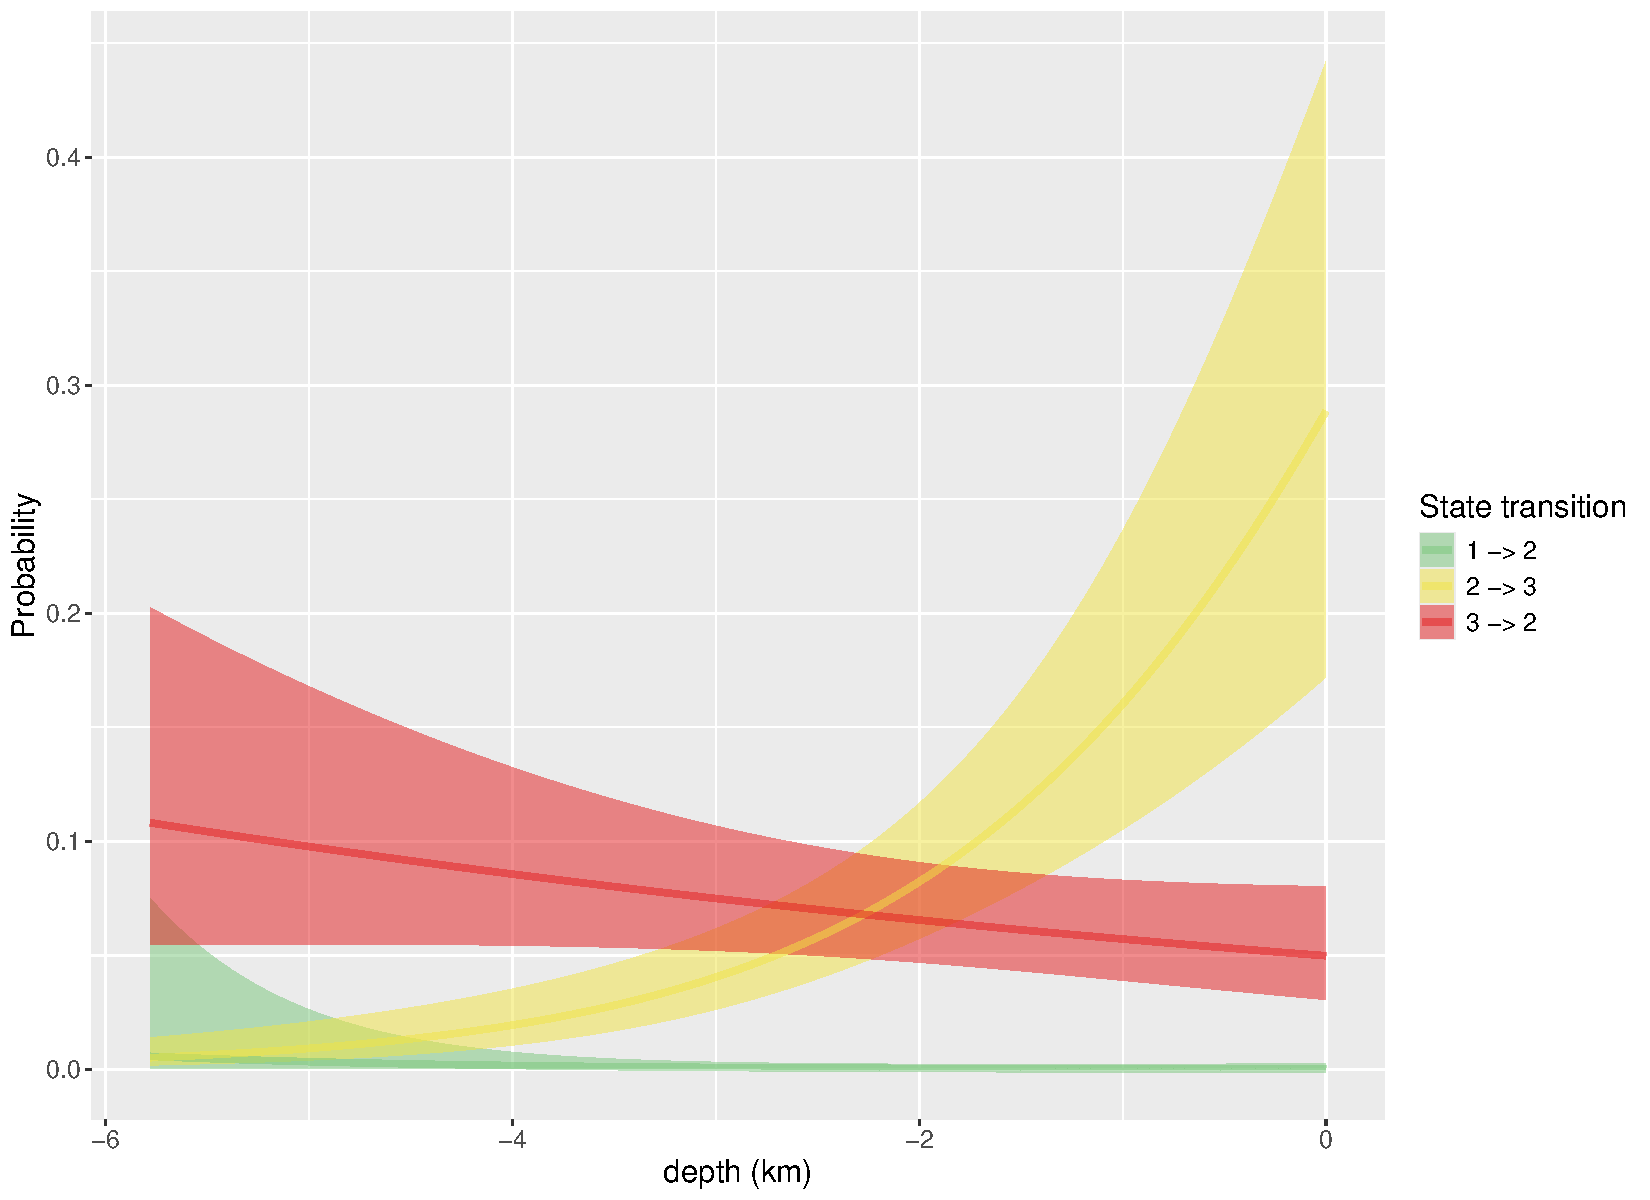
\includegraphics[width=0.9\textwidth]{../examples/ses/gammaBath.pdf}
    \caption{Southern elephant seal state transition probabilities (and 95\% confidence bands) as a function of sea floor depth (km) for switches from state 1 to state 2 (``1 -> 2''; green), from state 2 to state 3 (``2 -> 3''; yellow), and from state 3 to state 2 (``3 -> 2''; red).
    For calculating the probability of transitioning from state 1 to 2, the means of the other covariates were used.}
    \label{fig:gammaBath}
\end{figure}

%\begin{figure}
%    \centering
%    \includegraphics[width=0.8\textwidth]{fisherOrigSTcor_H&F.pdf}
%    \caption{Circular box plots of the step lengths and turn angles for the fisher data. For each of the five step length quantiles, a box plot of the corresponding angles is shown. Outliers (i.e., values outside 1.5 times the inter quartile range) are marked in red. Plot recreated using data and code provided by \cite{hodel2022circular}.}
%    \label{fig:fisherOrigSTcor}
%\end{figure}

\clearpage

\bibliographystyle{mee}
\bibliography{master}

\end{document}
